\documentclass[compress,red]{beamer}
\mode<presentation>
\setbeamertemplate{navigation symbols}{}

\usepackage{pgfpages}
\usepackage{color}
\usepackage{transparent}

% \setbeameroption{show notes}
% \setbeameroption{show notes on second screen=right}


\usetheme{Warsaw}
\setbeamercolor{uppercolgreen}{fg=white,bg=green!35}
\setbeamercolor{lowercolgreen}{fg=black,bg=green!10}



%\hypersetup{pdfpagemode=FullScreen} % makes your presentation go automatically to full screen

% define your own colors:
\definecolor{Red}{rgb}{1,0,0}
\definecolor{Blue}{rgb}{0,0,1}
\definecolor{Green}{rgb}{0,1,0}
\definecolor{magenta}{rgb}{1,0,.6}
\definecolor{lightblue}{rgb}{0,.5,1}
\definecolor{lightpurple}{rgb}{.6,.4,1}
\definecolor{gold}{rgb}{.6,.5,0}
\definecolor{orange}{rgb}{1,0.4,0}
\definecolor{hotpink}{rgb}{1,0,0.5}
\definecolor{newcolor2}{rgb}{.5,.3,.5}
\definecolor{newcolor}{rgb}{0,.3,1}
\definecolor{newcolor3}{rgb}{1,0,.35}
\definecolor{darkgreen1}{rgb}{0, .35, 0}
\definecolor{darkgreen}{rgb}{0, .6, 0}
\definecolor{darkred}{rgb}{.75,0,0}

\xdefinecolor{olive}{cmyk}{0.64,0,0.95,0.4}
\xdefinecolor{purpleish}{cmyk}{0.75,0.75,0,0}


\useoutertheme[subsection=false]{smoothbars}


% include packages
\usepackage{subfigure}
\usepackage{multicol}
\usepackage{amsmath}
\usepackage{epsfig}
\usepackage{graphicx}
\usepackage[all,knot]{xy}

\xyoption{arc}
\usepackage{url}
\usepackage{multimedia}
\usepackage{hyperref}
\usepackage{helvet}
\usepackage[polish,english]{babel}
\usepackage[utf8]{inputenc}
\usepackage{multirow}

\newcommand{\backupbegin}{
   \newcounter{framenumberappendix}
   \setcounter{framenumberappendix}{\value{framenumber}}
}
\newcommand{\backupend}{
   \addtocounter{framenumberappendix}{-\value{framenumber}}
   \addtocounter{framenumber}{\value{framenumberappendix}} 
}

% \setbeamertemplate{title page}[default]
% \setbeamercolor{title}{bg=}


% \setbeamertemplate{blocks}[default]
% \setbeamercolor{block title}{bg=}
% \setbeamercolor{block body}{bg=white}


%%%%%%%%%%%%5
%\usepackage{geometry}
%\geometry{verbose,letterpaper}
%\usepackage{movie15}
%\usepackage{hyperref}
%%%%%%%

% greetings, introduce yourself


%  \includegraphics[height=5cm]{fig/WRlogo.ps}


\title[White Rabbit @ CNGS \hspace{2em}\insertframenumber/\inserttotalframenumber]
{Performance results of \\the first White Rabbit installation for \\CNGS time transfer}

\institute{

   \begin{center}
    Hardware and Timing Section / ~~~ Institute of Electronic Systems \\
    ~~~~~~~~~~~~~~~~~~~~~CERN ~~~~~~~~~~~~~~~~ / ~~ Warsaw University of Technology \\
   \end{center}
%    \begin{center}
% 
%       Warsaw University of Technology \\
%       Hardware and Timing, CERN \\
%       University College London \\
%       University of Pavia \\
% 
%    \end{center}

}

\author[Maciej Lipi\'{n}ski]{\underline{Maciej~Lipi\'{n}ski},\and Tomasz~Wlostowski,\and 
Javier~Serrano,\and Pablo~Alvarez,\and David~Cobas,\and Alessandro~Rubini,\and Pedro~Moreira}

% \author{
% Maciej Lipi\'{n}ski 
% % on behalf of Maciej Lipi\'{n}ski 
% % Tomasz Wlostowski,
% % Javier Serrano, 
% % Pablo Alvarez, 
% % Juan David Gonzalez Cobas,
% % Alessandro Rubini and
% % Pedro Moreira
% }
\date{26th September 2012 \\ ISPCS 2012}



\pgfdeclareimage[height=0.6cm]{wr-logo}{../../figures/logo/WRlogo.ps}
\logo{\pgfuseimage{wr-logo}}
\AtBeginSection[]

\begin{document}

\frame{\titlepage}
%%%%%%%%%%%%%%%%%%%%%%%%%%%%%%%%%%%%%%%%%%%%%%%%%%%%%%%%%%%%%%%%%%%%%%%%%%%%%%%%%%%%%%%%%%%%%%%%%%%%
% \setbeamertemplate{background}{\includegraphics[width=0.95\paperwidth]{figs/neutrino_joke.eps}} 
\begin{frame}<beamer>{Outline}
    \tableofcontents %[currentsection]

\end{frame}
% \setbeamertemplate{background}{} 

%%%%%%%%%%%%%%%%%%%%%%%%%%%%%%%%%%%%%%%%%%%%%%%%%%%%%%%%%%%%%%%%%%%%%%%%%%%%%%%%%%%%%%%%%%%%%%%%%%%%
\section{Introduction}
\subsection{}
%%%%%%%%%%%%%%%%%%%%%%%%%%%%%%%%%%%%%%%%%%%%%%%%%%%%%%%%%%%%%%%%%%%%%%%%%%%%%%%%%%%%%%%%%%%%%%%%%%%%
\setbeamertemplate{background}{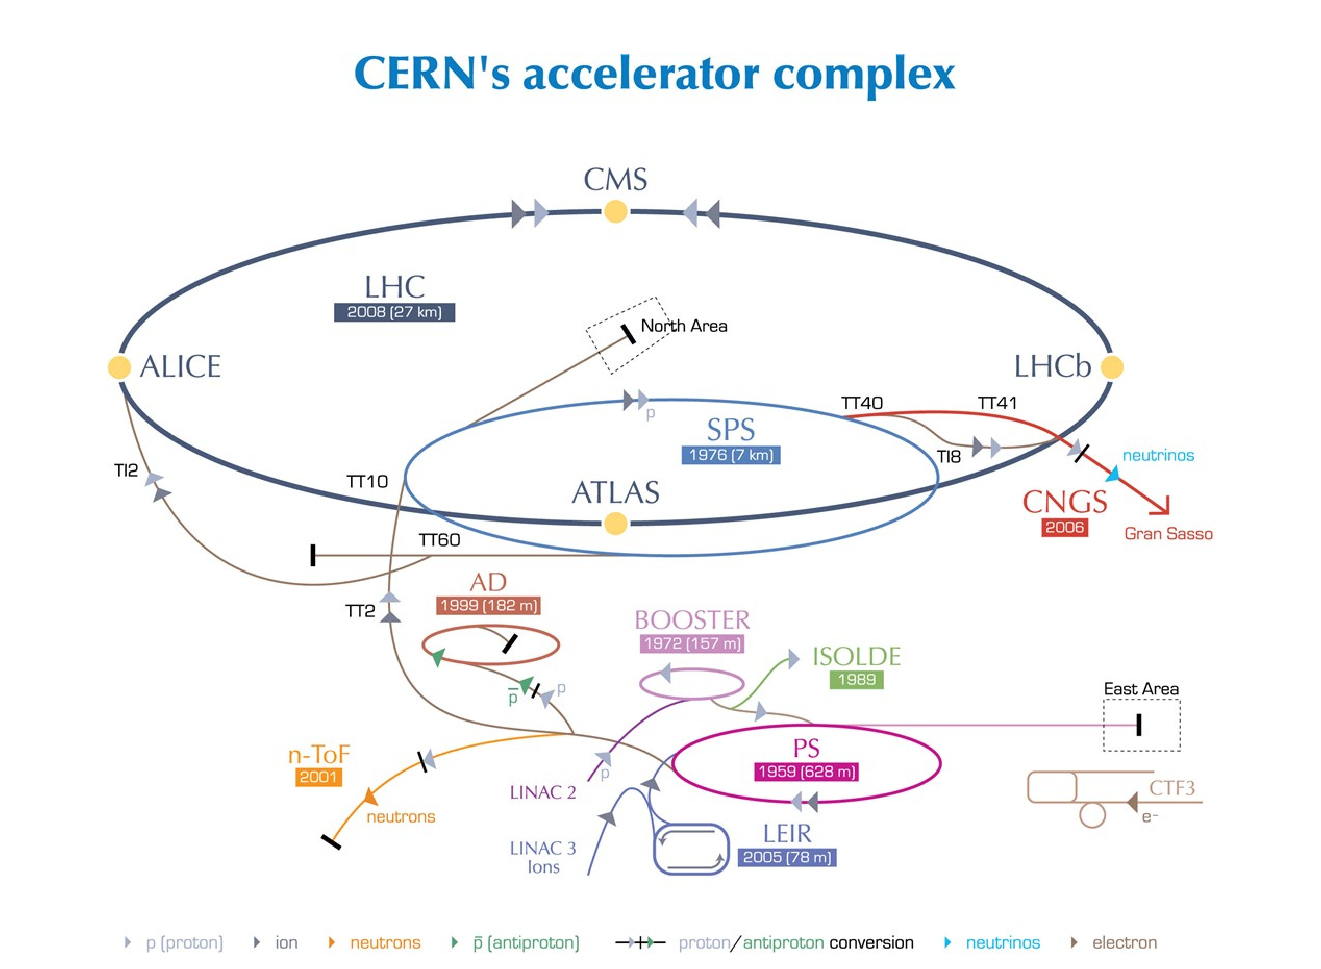
\includegraphics[width=0.95\paperwidth]{figs/accelerators_background.eps}} 
%  \addtobeamertemplate{block begin}{\pgfsetfillopacity{0.5}}{\pgfsetfillopacity{0.5}}
%  \addtobeamertemplate{block alerted begin}{\pgfsetfillopacity{0.5}}{\pgfsetfillopacity{1}}
%  \addtobeamertemplate{block example begin}{\pgfsetfillopacity{0.5}}{\pgfsetfillopacity{1}}
\begin{frame}{Introduction}

% \pause
% \begin{columns}[c]
%    \column{0.01\textwidth}
%   \column{0.55\textwidth}
% 
%      \begin{block}{Hardware \& Timing Section:} 
% 	\begin{itemize}
% 	  \item synchronization and control
% 	  \item \textbf{White Rabbit} -- PTP-based control and timing 
% 	  \item Time transfer for \textbf{CNGS}
% 	\end{itemize}
%      \end{block}
% 
%   \column{0.6\textwidth}
%     \begin{center}
% 
% %       \includegraphics<1-3>[width=6.5cm]{../../figures/applications/CERN/accelerators.eps}
%       \includegraphics<3>[width=6.0cm]{figs/cngs-overview.v2.eps}
%     \end{center}
% \end{columns}

\end{frame}
\setbeamertemplate{background}{} 
%%%%%%%%%%%%%%%%%%%%%%%%%%%%%%%%%%%%%%%%%%%%%%%%%%%%%%%%%%%%%%%%%%%%%%%%%%%%%%%%%%%%%%%%%%%%%%%%%%%%
% \section{Introduction}
% \subsection{}
%%%%%%%%%%%%%%%%%%%%%%%%%%%%%%%%%%%%%%%%%%%%%%%%%%%%%%%%%%%%%%%%%%%%%%%%%%%%%%%%%%%%%%%%%%%%%%%%%%%%
\setbeamertemplate{background}{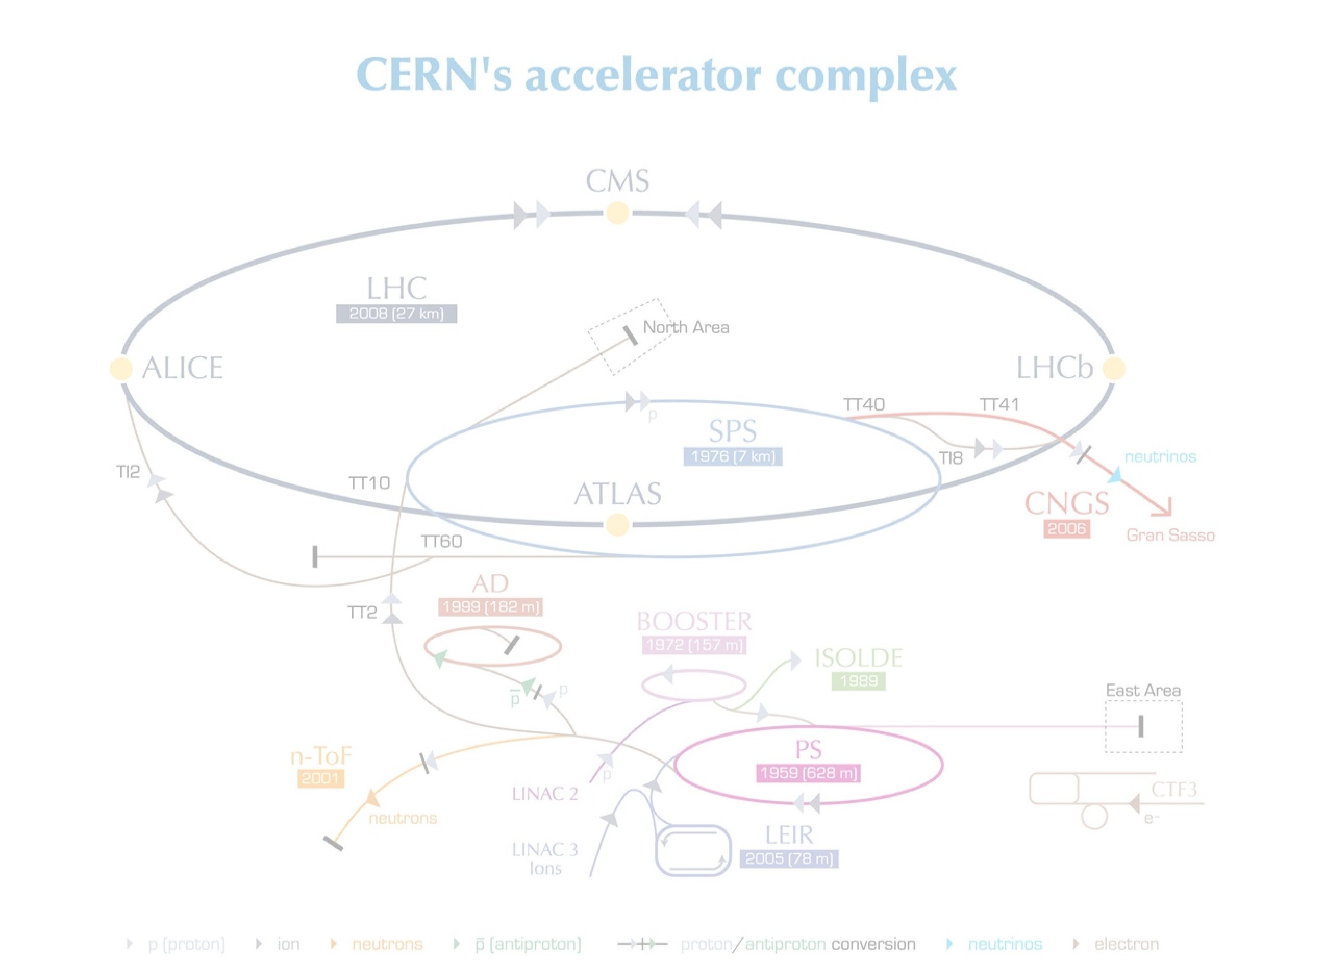
\includegraphics[width=0.95\paperwidth]{figs/accelerators_background2.eps}} 
%  \addtobeamertemplate{block begin}{\pgfsetfillopacity{0.5}}{\pgfsetfillopacity{0.5}}
%  \addtobeamertemplate{block alerted begin}{\pgfsetfillopacity{0.5}}{\pgfsetfillopacity{1}}
%  \addtobeamertemplate{block example begin}{\pgfsetfillopacity{0.5}}{\pgfsetfillopacity{1}}
\begin{frame}{Introduction}

\begin{columns}[c]
   \column{0.01\textwidth}
  \column{0.55\textwidth}

     \begin{block}{Hardware \& Timing Section:} 
	\begin{itemize}
	  \item synchronization and control
	  \item \textbf{White Rabbit} -- PTP-based control and timing 
	  \item Time transfer for \textbf{CNGS}
	\end{itemize}
     \end{block}

  \column{0.6\textwidth}
    \begin{center}
\pause
%       \includegraphics<1-3>[width=6.5cm]{../../figures/applications/CERN/accelerators.eps}
      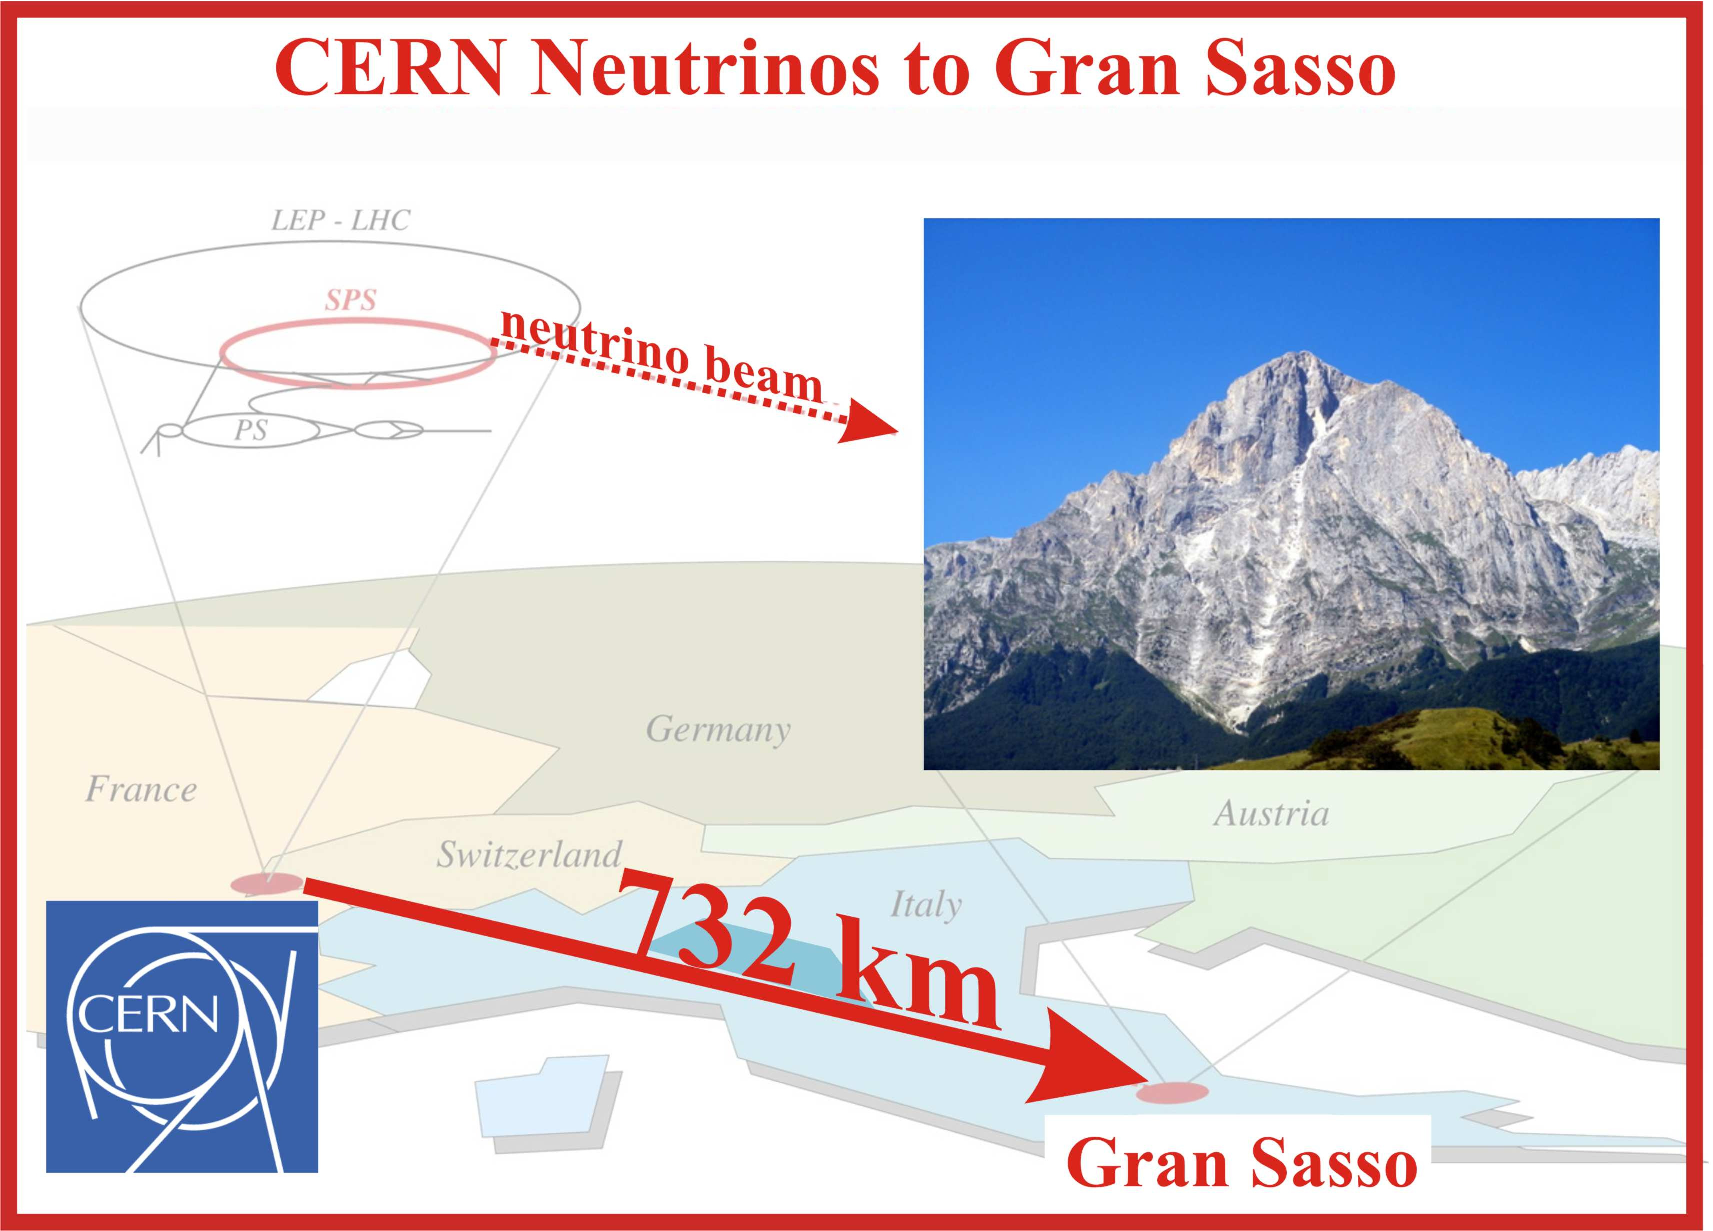
\includegraphics[width=6.0cm]{figs/cngs-overview.v3.eps}
    \end{center}
\end{columns}

\end{frame}
\setbeamertemplate{background}{} 

% %%%%%%%%%%%%%%%%%%%%%%%%%%%%%%%%%%%%%%%%%%%%%%%%%%%%%%%%%%%%%%%%%%%%%%%%%%%%%%%%%%%%%%%%%%%%%%%%%%%%
% \section{Introduction}
% \subsection{}
% %%%%%%%%%%%%%%%%%%%%%%%%%%%%%%%%%%%%%%%%%%%%%%%%%%%%%%%%%%%%%%%%%%%%%%%%%%%%%%%%%%%%%%%%%%%%%%%%%%%%
% \setbeamertemplate{background}{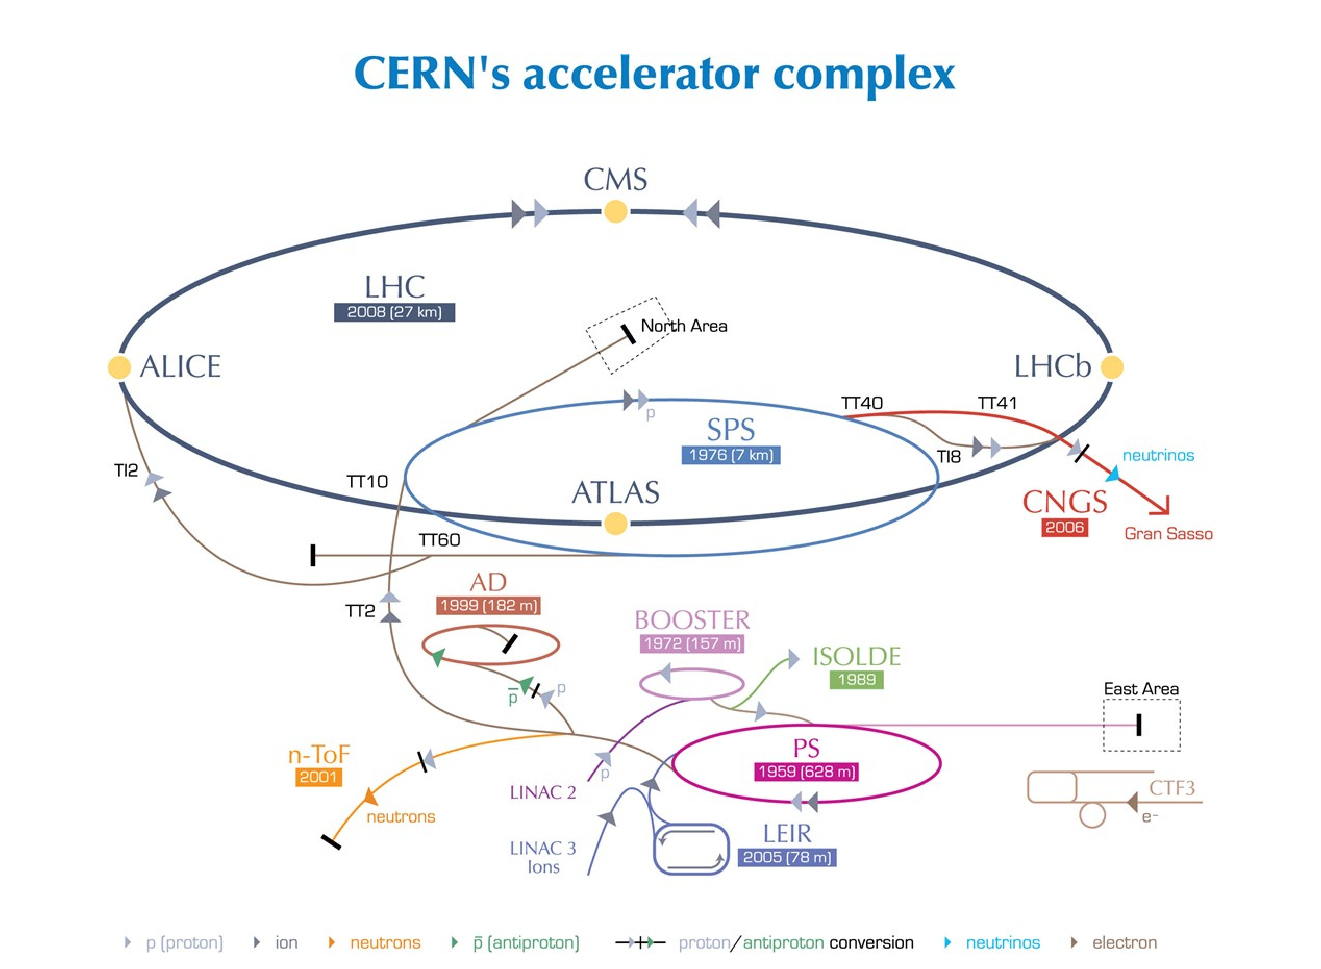
\includegraphics[width=\paperwidth]{figs/accelerators_background.eps}} 
% 
% \begin{frame}{Introduction}
% 
% \pause
% \begin{columns}[c]
%   \column{0.55\textwidth}
%     \begin{center}
%      \textbf{Hardware \& Timing Section:} \\
%       \begin{itemize}
% 	\item<1-4> synchronization and control of accelerator devices 
% 	\item<2-4> \textbf{White Rabbit} -- new PTP-based control and timing 
% % 	  \begin{center}
% % 	    \includegraphics<2>[width=1.5cm]{../../figures/logo/WRlogo.ps}
% % 	  \end{center}
% %         \vspace{-0.7cm}
% 	\item<3-4> Time transfer for \textbf{CERN Neutrino to Gran Sasso (CNGS)} experiment
%       \end{itemize}
% 
%     \end{center}
%   \column{0.6\textwidth}
%     \begin{center}
% %       \includegraphics<1-3>[width=6.5cm]{../../figures/applications/CERN/accelerators.eps}
%       \includegraphics<4>[width=6.5cm]{figs/cngs-general.eps}
%     \end{center}
% \end{columns}
% 
% \end{frame}
% \setbeamertemplate{background}{} 

%%%%%%%%%%%%%%%%%%%%%%%%%%%%%%%%%%%%%%%%%%%%%%%%%%%%%%%%%%%%%%%%%%%%%%%%%%%%%%%%%%%%%%%%%%%%%%%%%%%%
% \section{Introduction}
% \subsection{}
%%%%%%%%%%%%%%%%%%%%%%%%%%%%%%%%%%%%%%%%%%%%%%%%%%%%%%%%%%%%%%%%%%%%%%%%%%%%%%%%%%%%%%%%%%%%%%%%%%%%
\begin{frame}{Title explained}

\begin{columns}[c]
  \column{0.5\textwidth}
    \begin{center}
	\textbf{Performance results of \\White Rabbit installation for \\CNGS time transfer}
    \end{center}
  \column{0.5\textwidth}
    \begin{center}
      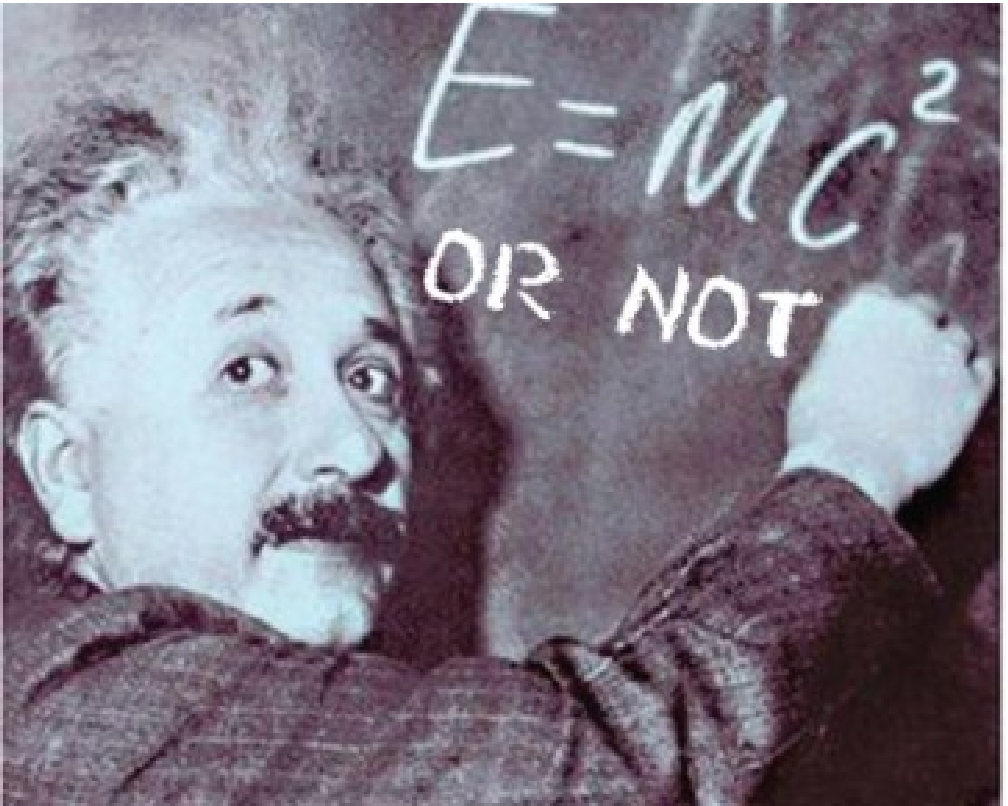
\includegraphics[width=4.0cm]{figs/emc2.eps}
    \end{center}
\end{columns}

\end{frame}
%%%%%%%%%%%%%%%%%%%%%%%%%%%%%%%%%%%%%%%%%%%%%%%%%%%%%%%%%%%%%%%%%%%%%%%%%%%%%%%%%%%%%%%%%%%%%%%%%%%%
\section{White Rabbit}
\subsection{}
%%%%%%%%%%%%%%%%%%%%%%%%%%%%%%%%%%%%%%%%%%%%%%%%%%%%%%%%%%%%%%%%%%%%%%%%%%%%%%%%%%%%%%%%%%%%%%%%%%%%
\begin{frame}{What is White Rabbit?}

\begin{columns}[c]
	\column{0.8\textwidth}
	  \begin{itemize}
		\item Accelerator's control and timing
		\item Based on well-known technologies
		\item Open Hardware and Open Software
		\item International collaboration
		\item Main features:
		\begin{itemize}
		  \item transparent,  {\bf high-accuracy} synchronization
		  \item low-latency,  {\bf deterministic} data delivery
		  \item designed for  {\bf high reliability}
% 		  \item plug \& play
		\end{itemize}
	  \end{itemize}
	\column{0.3\textwidth}
		\begin{center}
% 		\pause
		\hspace{-0.5cm}
		\includegraphics<1>[width=1.1\textwidth]{../../figures/logo/WRlogo.ps}
		\includegraphics<2>[width=1.1\textwidth]{../../figures/misc/rabbit.eps}
		\end{center}
	\end{columns}

\end{frame}
%%%%%%%%%%%%%%%%%%%%%%%%%%%%%%%%%%%%%%%%%%%%%%%%%%%%%%%%%%%%%%%%%%%%%%%%%%%%%%%%%%%%%%%%%%%%%%%%%%%%
% \section{White Rabbit}
% \subsection{}
%%%%%%%%%%%%%%%%%%%%%%%%%%%%%%%%%%%%%%%%%%%%%%%%%%%%%%%%%%%%%%%%%%%%%%%%%%%%%%%%%%%%%%%%%%%%%%%%%%%%
\setbeamertemplate{background}{\includegraphics[width=0.95\paperwidth]{figs/syncE.v2.eps}} 
\begin{frame}{Time Distribution with White Rabbit}


\begin{columns}[c]
\column{0.01\textwidth}
\column{0.99\textwidth}
  \begin{itemize}
    \item Synchronization with {\bf sub-ns} accuracy and {\bf ps} precision
    \item Combination of
	\begin{itemize}\small
	  \item Precision Time Protocol ({\bf PTP}) synchronization
	  \item Synchronous Ethernet ({\bf SyncE}) syntonization
	  \item Digital Dual-Mixer Time Difference ({\bf DDMTD}) phase detection
	\end{itemize}
  \end{itemize}
  \begin{center}
  \vspace{6.7cm}
%   \vspace{-3cm}
%   \includegraphics<1>[width=1.0\textwidth]{figs/syncE.eps}
%   \includegraphics<2>[width=1.0\textwidth]{figs/ddmtd.eps}

%   \includegraphics<1>[height=0.5\textheight]{figs/syncE.eps}
%   \includegraphics<2>[height=0.5\textheight]{figs/ddmtd.eps}
  \end{center}  
\end{columns}

\end{frame}
\setbeamertemplate{background}{} 
%%%%%%%%%%%%%%%%%%%%%%%%%%%%%%%%%%%%%%%%%%%%%%%%%%%%%%%%%%%%%%%%%%%%%%%%%%%%%%%%%%%%%%%%%%%%%%%%%%%%
% \section{White Rabbit}
% \subsection{}
%%%%%%%%%%%%%%%%%%%%%%%%%%%%%%%%%%%%%%%%%%%%%%%%%%%%%%%%%%%%%%%%%%%%%%%%%%%%%%%%%%%%%%%%%%%%%%%%%%%%
\setbeamertemplate{background}{\includegraphics[width=0.95\paperwidth]{figs/ddmtd.v2.eps}} 
\begin{frame}{Time Distribution with White Rabbit}

\begin{columns}[c]
\column{0.01\textwidth}
\column{0.99\textwidth}

  \begin{itemize}
    \item Synchronization with {\bf sub-ns} accuracy and {\bf ps} precision
    \item Combination of
	\begin{itemize}\small
	  \item Precision Time Protocol ({\bf PTP}) synchronization
	  \item Synchronous Ethernet ({\bf SyncE}) syntonization
	  \item Digital Dual-Mixer Time Difference ({\bf DDMTD}) phase detection
	\end{itemize}
  \end{itemize}
  \begin{center}
  \vspace{6.9cm}
\hspace{2cm}
%   \vspace{-3cm}
%   \includegraphics<1>[width=1.0\textwidth]{figs/syncE.eps}
%   \includegraphics<2>[width=1.0\textwidth]{figs/ddmtd.eps}

%   \includegraphics<1>[height=0.5\textheight]{figs/syncE.eps}
%   \includegraphics<2>[height=0.5\textheight]{figs/ddmtd.eps}
  \end{center}  
\end{columns}

\end{frame}
\setbeamertemplate{background}{} 
%%%%%%%%%%%%%%%%%%%%%%%%%%%%%%%%%%%%%%%%%%%%%%%%%%%%%%%%%%%%%%%%%%%%%%%%%%%%%%%%%%%%%%%%%%%%%%%%%%%%
% \section{White Rabbit}
% \subsection{}
%%%%%%%%%%%%%%%%%%%%%%%%%%%%%%%%%%%%%%%%%%%%%%%%%%%%%%%%%%%%%%%%%%%%%%%%%%%%%%%%%%%%%%%%%%%%%%%%%%%%
\begin{frame}{Extension to PTP: WR PTP}
	\begin{itemize}
	  \item Addresses PTP's limitations
	  \item Compatible with "standard" PTP gear
	  \item Ongoing standardization effort
	\end{itemize}
\end{frame}
%%%%%%%%%%%%%%%%%%%%%%%%%%%%%%%%%%%%%%%%%%%%%%%%%%%%%%%%%%%%%%%%%%%%%%%%%%%%%%%%%%%%%%%%%%%%%%%%%%%%
\section{CNGS}
\subsection{}
%%%%%%%%%%%%%%%%%%%%%%%%%%%%%%%%%%%%%%%%%%%%%%%%%%%%%%%%%%%%%%%%%%%%%%%%%%%%%%%%%%%%%%%%%%%%%%%%%%%%
\begin{frame}{CERN Neutrinos to Gran Sasso (CNGS)}

    \begin{center}
      \includegraphics[width=0.9\textwidth]{figs/cngs-general.v2.eps}
    \end{center}

    \begin{center}
      \begin{itemize}
	\item Investigation of neutrino oscillation
	\item Time of Flight (ToF) measurement
% 	\item Experiment repeated confirm error
% 	\item First deployment of \textbf{White Rabbit PTP-base system} 
      \end{itemize}

    \end{center}


\end{frame}
%%%%%%%%%%%%%%%%%%%%%%%%%%%%%%%%%%%%%%%%%%%%%%%%%%%%%%%%%%%%%%%%%%%%%%%%%%%%%%%%%%%%%%%%%%%%%%%%%%%%
% \section{CNGS}
% \subsection{}
%%%%%%%%%%%%%%%%%%%%%%%%%%%%%%%%%%%%%%%%%%%%%%%%%%%%%%%%%%%%%%%%%%%%%%%%%%%%%%%%%%%%%%%%%%%%%%%%%%%%
\begin{frame}{CERN Neutrinos to Gran Sasso (CNGS)}

      \begin{center}
      
      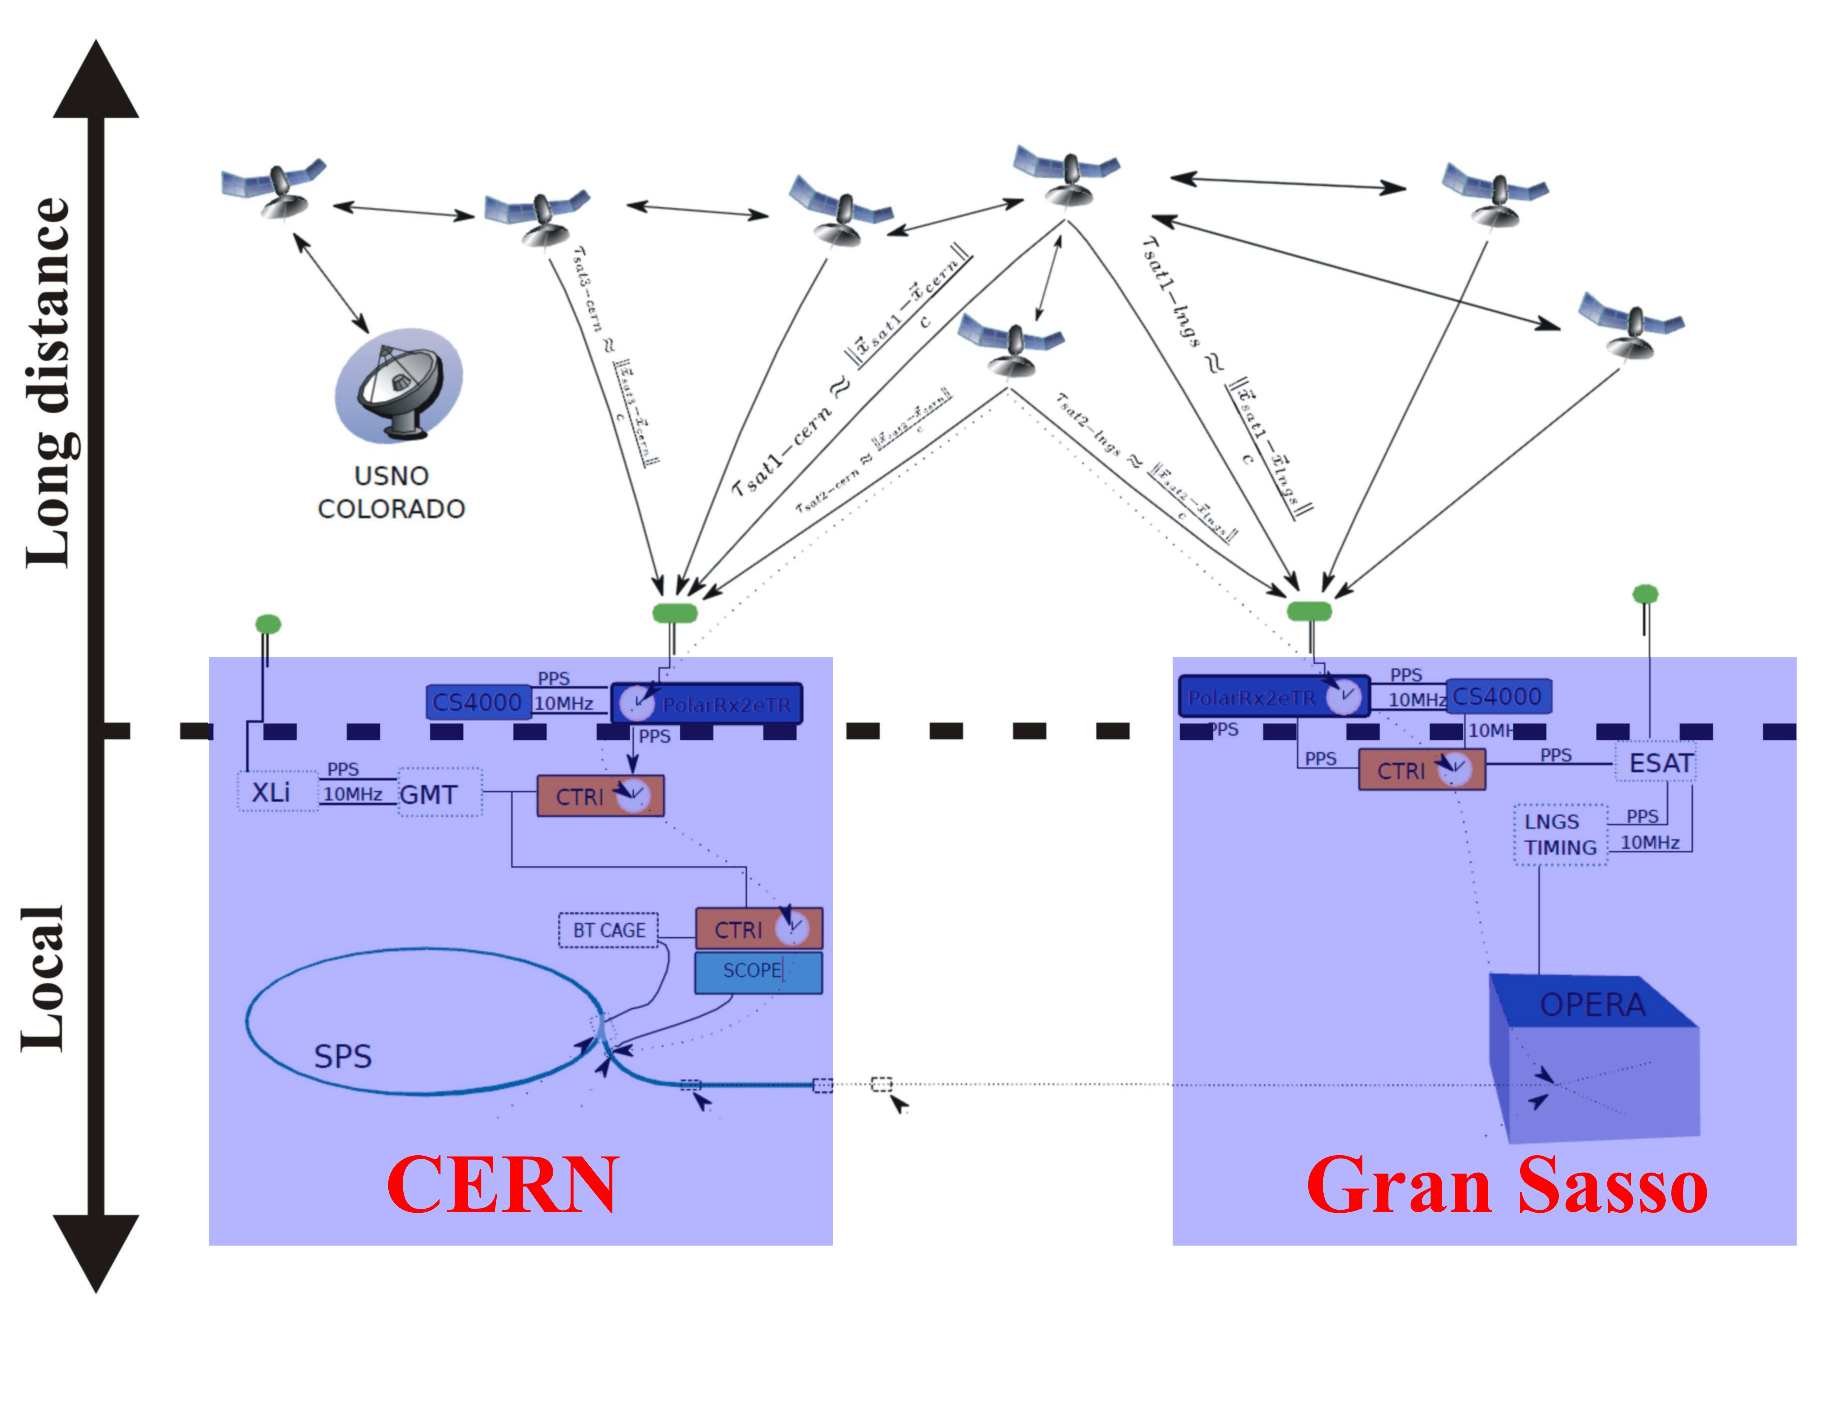
\includegraphics[width=0.9\textwidth]{figs/cngs-timing-1.v2.eps} 
%       \includegraphics<3>[width=1.2\textwidth]{figs/cngs-detailed-2.eps}
%       \includegraphics<3>[width=1.0\textwidth]{figs/cngs-detailed-new.eps}
      \end{center}

\end{frame}
%%%%%%%%%%%%%%%%%%%%%%%%%%%%%%%%%%%%%%%%%%%%%%%%%%%%%%%%%%%%%%%%%%%%%%%%%%%%%%%%%%%%%%%%%%%%%%%%%%%%
% \section{White Rabbit}
% \subsection{}
%%%%%%%%%%%%%%%%%%%%%%%%%%%%%%%%%%%%%%%%%%%%%%%%%%%%%%%%%%%%%%%%%%%%%%%%%%%%%%%%%%%%%%%%%%%%%%%%%%%%
\begin{frame}{Old CNGS time transfer}

      \begin{center}
      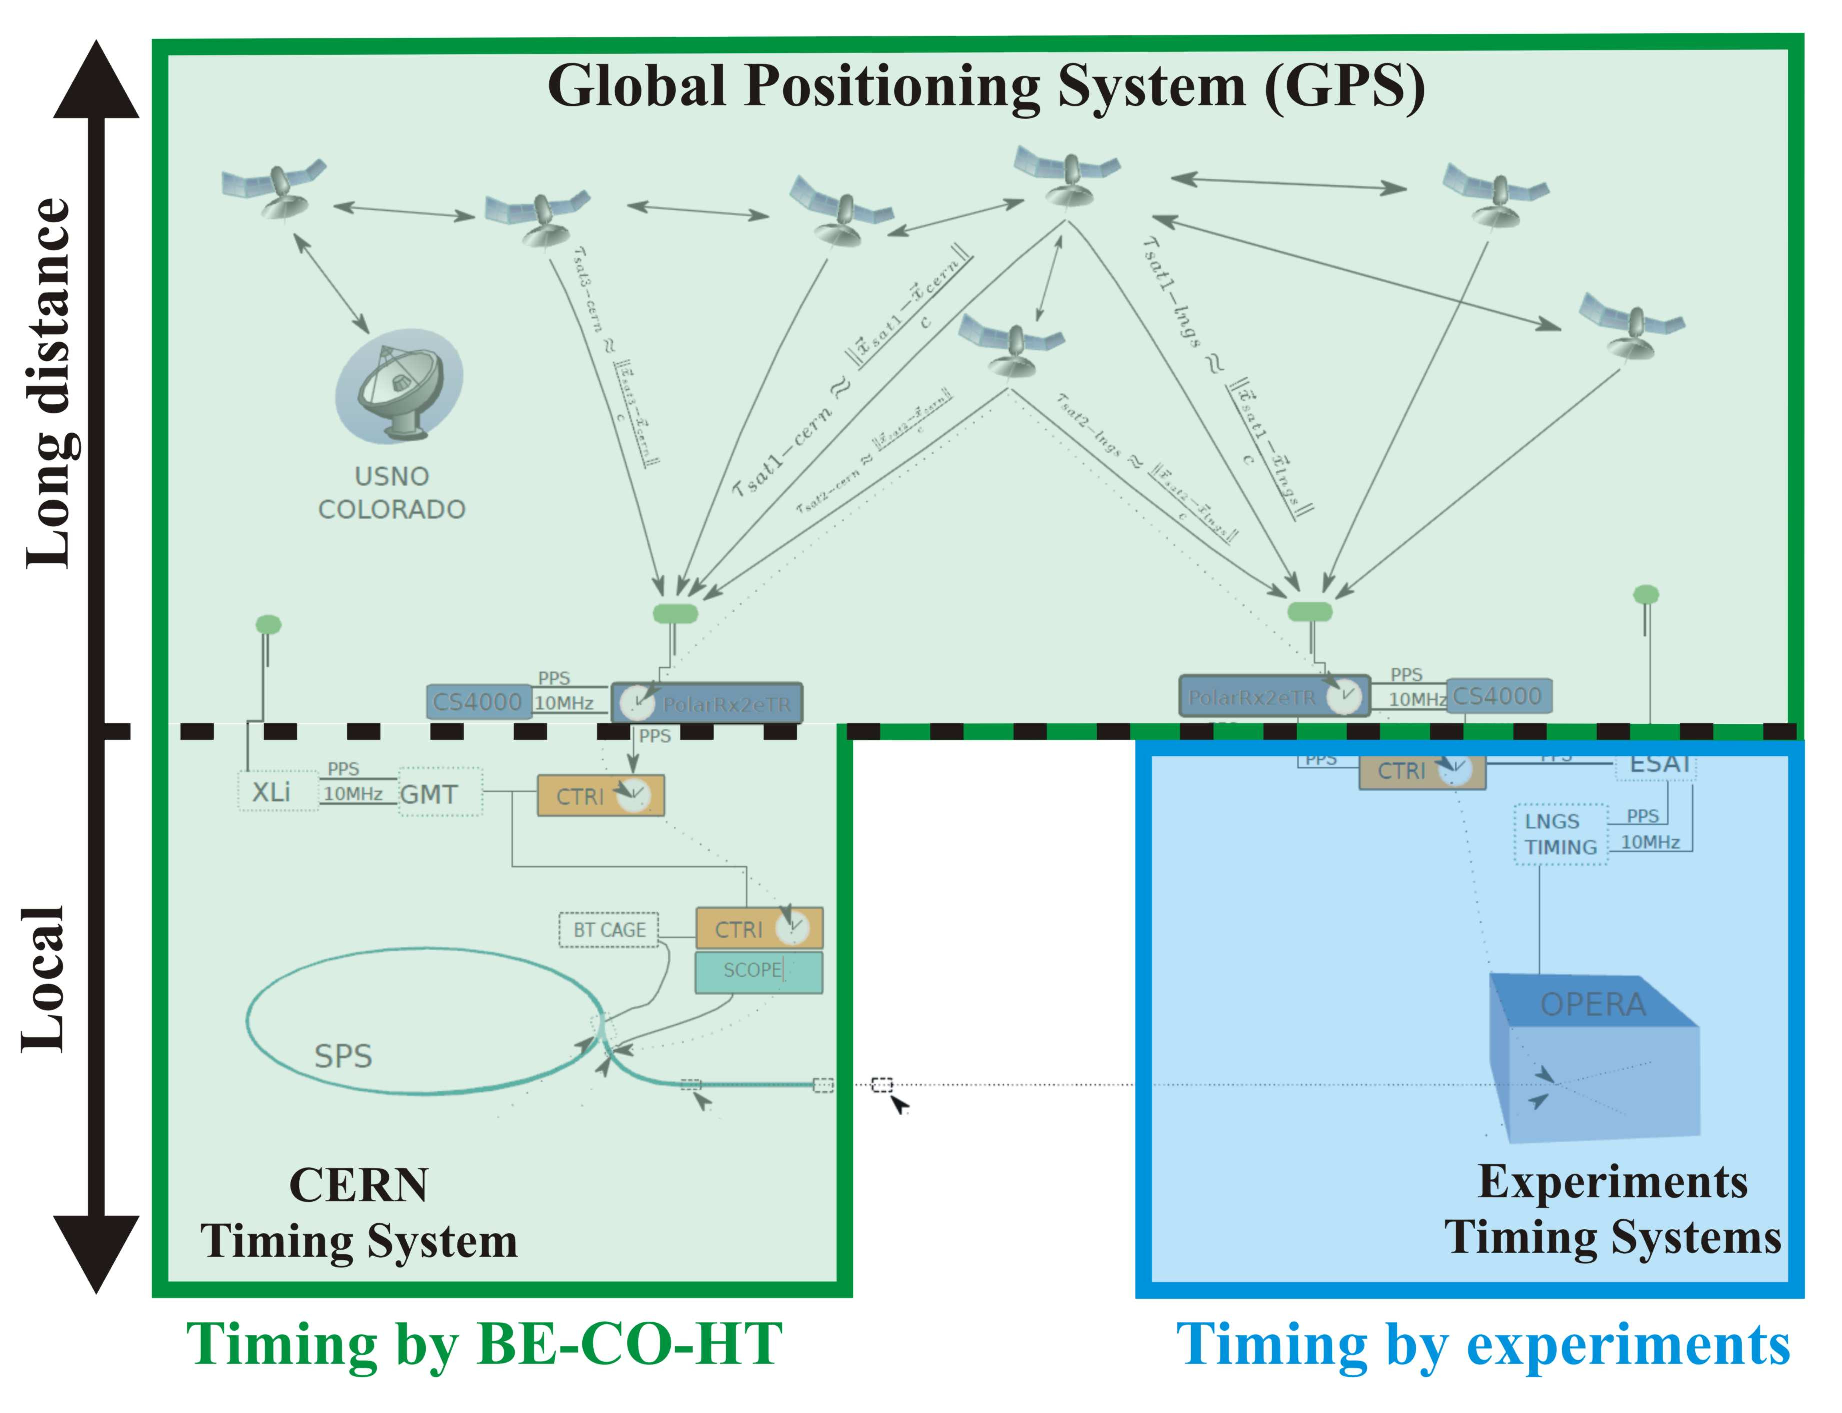
\includegraphics[width=0.9\textwidth]{figs/cngs-timing-2.eps}
      \end{center}

\end{frame}
%%%%%%%%%%%%%%%%%%%%%%%%%%%%%%%%%%%%%%%%%%%%%%%%%%%%%%%%%%%%%%%%%%%%%%%%%%%%%%%%%%%%%%%%%%%%%%%%%%%%
% \section{White Rabbit}
% \subsection{}
%%%%%%%%%%%%%%%%%%%%%%%%%%%%%%%%%%%%%%%%%%%%%%%%%%%%%%%%%%%%%%%%%%%%%%%%%%%%%%%%%%%%%%%%%%%%%%%%%%%%
\begin{frame}{New time transfer with WR}

      \begin{center}
%       \vspace{-0.3cm}
      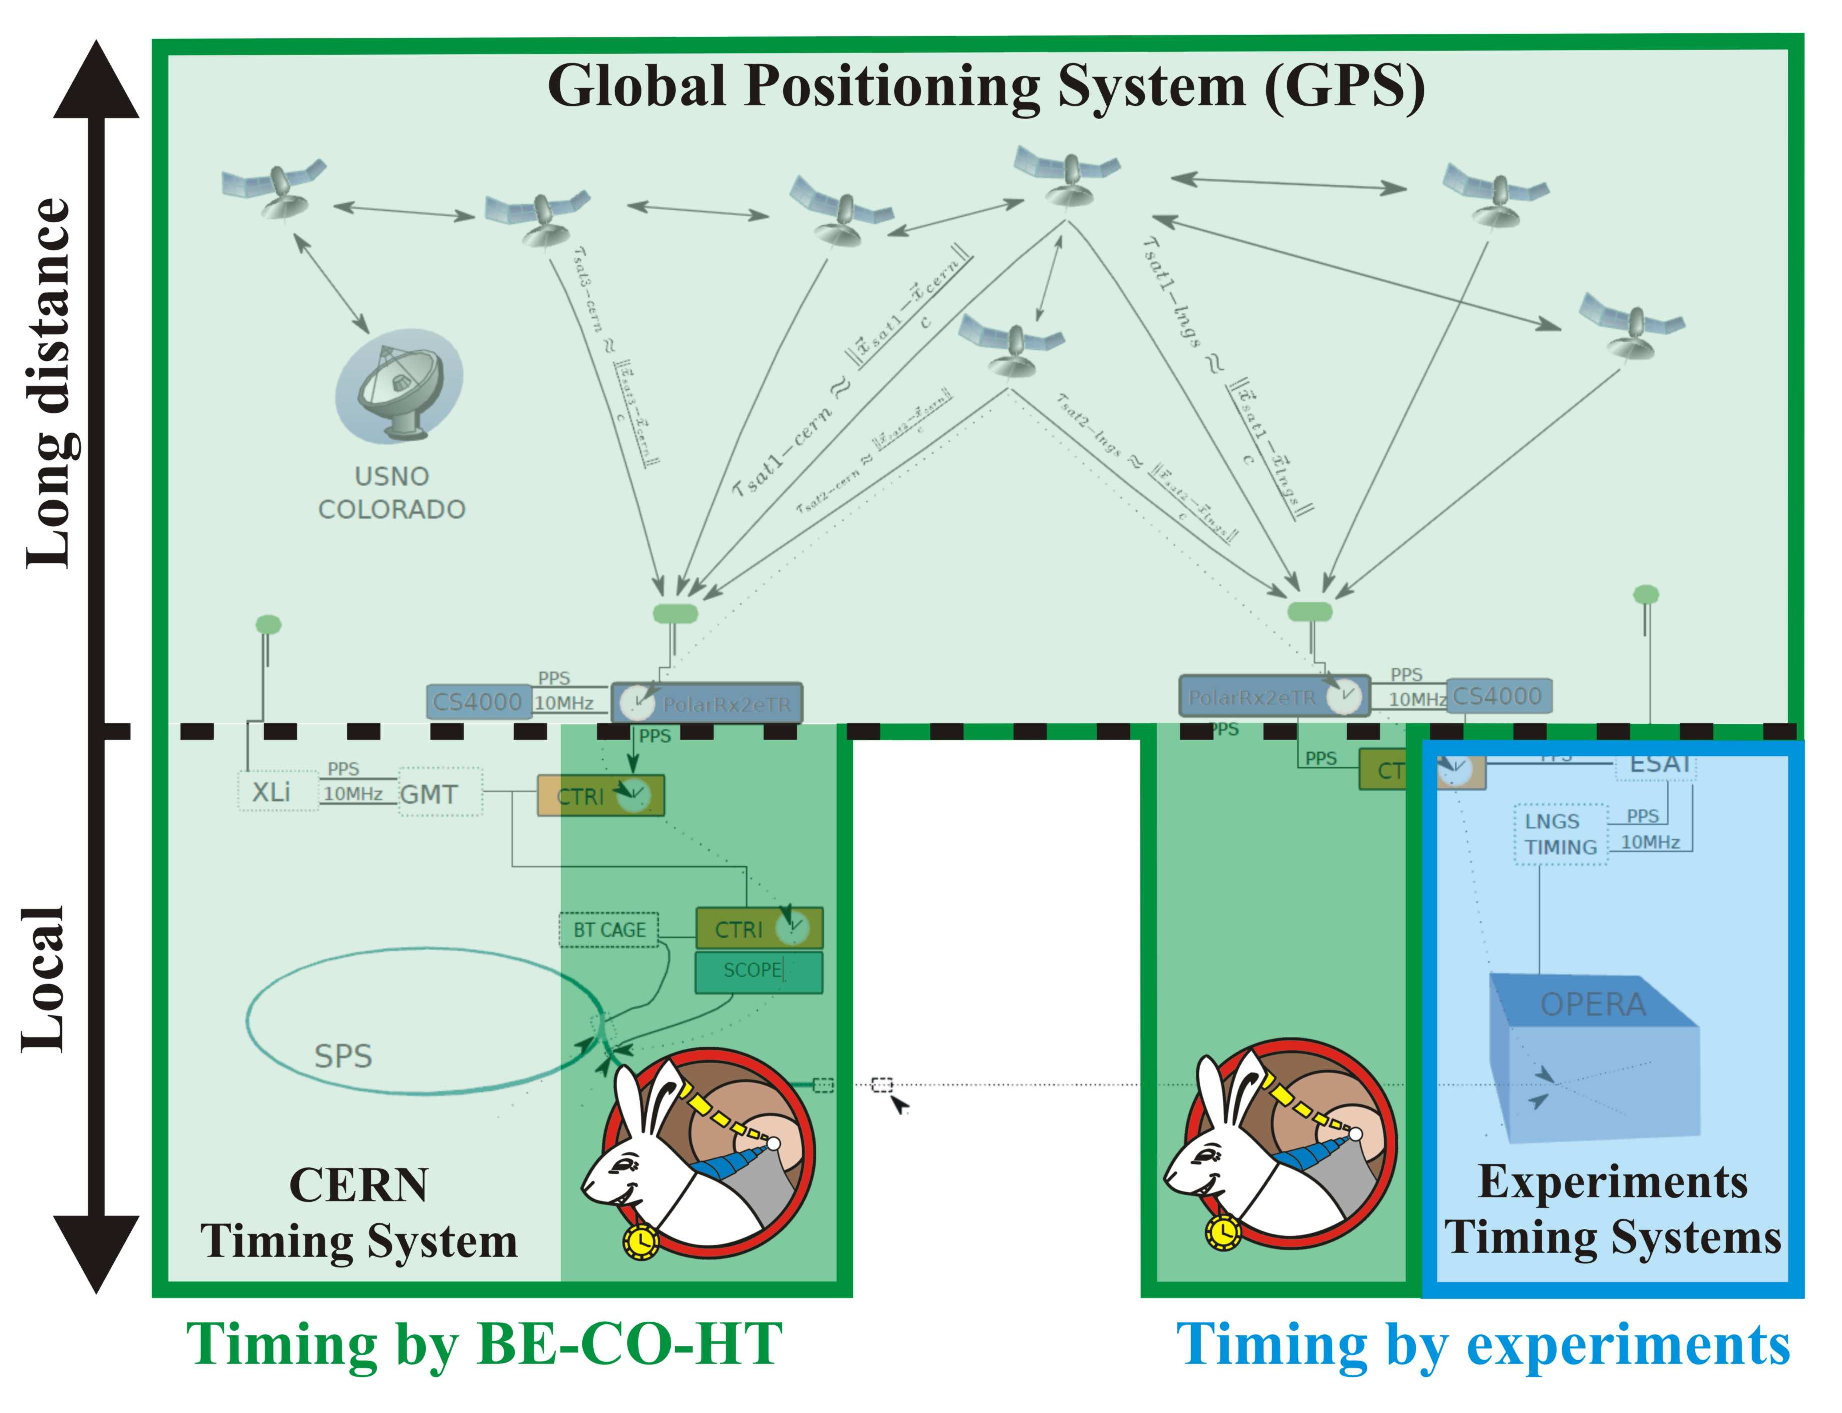
\includegraphics[width=0.9\textwidth]{figs/cngs-timing-3.eps}
%        \includegraphics<2>[width=0.75\textwidth]{../../figures/applications/OperaTiming2.eps}
      \end{center}

\end{frame}
%%%%%%%%%%%%%%%%%%%%%%%%%%%%%%%%%%%%%%%%%%%%%%%%%%%%%%%%%%%%%%%%%%%%%%%%%%%%%%%%%%%%%%%%%%%%%%%%%%%%
% \section{White Rabbit}
% \subsection{}
%%%%%%%%%%%%%%%%%%%%%%%%%%%%%%%%%%%%%%%%%%%%%%%%%%%%%%%%%%%%%%%%%%%%%%%%%%%%%%%%%%%%%%%%%%%%%%%%%%%%
\begin{frame}{WR installation}


  \begin{columns}[c]
	\column{0.7\textwidth}
	  \begin{itemize}
		\item Grandmaster WR Switch
		\item 8 km of fiber between switches
		\item Boundary Clock WR Switch
		\item WR Node -- includes Time-to-Digital Converter (TDC):
		\begin{itemize}
		  \item 55 ps precision (std. dev)
		  \item 300 ps accuracy
		\end{itemize}
		\item Performance monitoring
	  \end{itemize}
	\column{0.5\textwidth}
		\begin{center}
% 		\pause
		\vspace{-0.5cm}
		\includegraphics<1>[height=0.75\textheight]{figs/lngs_installation.eps}
		\includegraphics<2>[height=0.75\textheight]{figs/lngs_installation-dimmed.eps}
		\end{center}
  \end{columns}

\end{frame}
%%%%%%%%%%%%%%%%%%%%%%%%%%%%%%%%%%%%%%%%%%%%%%%%%%%%%%%%%%%%%%%%%%%%%%%%%%%%%%%%%%%%%%%%%%%%%%%%%%%%
\section{CNGS Measurements}
\subsection{}
%%%%%%%%%%%%%%%%%%%%%%%%%%%%%%%%%%%%%%%%%%%%%%%%%%%%%%%%%%%%%%%%%%%%%%%%%%%%%%%%%%%%%%%%%%%%%%%%%%%%
\begin{frame}{CNGS performance measurement (1)}

  \begin{columns}[c]
	\column{0.6\textwidth}
	  \begin{itemize}
		\item Duration: 31 d, 7 h, 40 s ($2.7*10^6$ samples)
		\item WR Nodes with TDC used
		\item Timestamping reference PPS
		\item Measurement includes inaccuracy of TDC
	  \end{itemize}
	\column{0.6\textwidth}
		\begin{center}
% 		\includegraphics[width=0.8\textwidth]{figs/performance_testing_setup.eps}
		\includegraphics[width=0.93\textwidth]{figs/performance_testing_setup-detail.v2.eps}
		\end{center}
  \end{columns}


\end{frame}
%%%%%%%%%%%%%%%%%%%%%%%%%%%%%%%%%%%%%%%%%%%%%%%%%%%%%%%%%%%%%%%%%%%%%%%%%%%%%%%%%%%%%%%%%%%%%%%%%%%%
% \section{CNGS Measurements}
% \subsection{}
%%%%%%%%%%%%%%%%%%%%%%%%%%%%%%%%%%%%%%%%%%%%%%%%%%%%%%%%%%%%%%%%%%%%%%%%%%%%%%%%%%%%%%%%%%%%%%%%%%%%
\begin{frame}{CNGS performance measurement (2)}

  \begin{columns}[c]
	\column{0.6\textwidth}
	  \begin{center}
	  Time Errors:
	  \end{center}
	  \begin{center}
	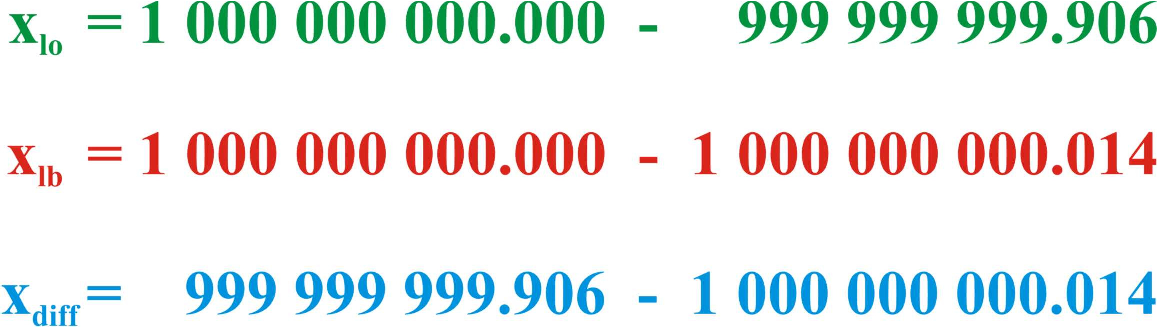
\includegraphics[width=0.93\textwidth]{figs/timeErrors.eps}
	  \end{center}
	\column{0.6\textwidth}
% 		\vspace{-0.4cm}
		\begin{center}
		\includegraphics[width=0.93\textwidth]{figs/performance_testing_setup-detail.v2.eps}
		
		\end{center}
  \end{columns}


\end{frame}
%%%%%%%%%%%%%%%%%%%%%%%%%%%%%%%%%%%%%%%%%%%%%%%%%%%%%%%%%%%%%%%%%%%%%%%%%%%%%%%%%%%%%%%%%%%%%%%%%%%%
% \section{CNGS Measurements}
% \subsection{}
%%%%%%%%%%%%%%%%%%%%%%%%%%%%%%%%%%%%%%%%%%%%%%%%%%%%%%%%%%%%%%%%%%%%%%%%%%%%%%%%%%%%%%%%%%%%%%%%%%%%
% \begin{frame}{CNGS performance measurement (2)}
% 
%   \begin{columns}[c]
% 	\column{0.6\textwidth}
% 	  \begin{center}
% 	      \begin{table}[!t]\tiny
% 	      \begin{tabular}{| l | c | c |}          \hline
% 	       \multicolumn{3}{|c|}{\textbf{Local PPS }}  \\   \hline
% 	      & \textbf{UTC} & \textbf{nanoseconds} \\   \hline
% 
% 	      1 & 1337380733 & 999999885.959 \\   \hline
% 	      2 & 1337380734 & 999999886.014 \\   \hline
% 	      3 & 1337380735 & 999999885.934 \\   \hline
% 	      4 & 1337380736 & 999999885.906 \\   \hline
% 		&      ...   &  ..           \\   \hline
% 	      2706160 & 1340086893 & 999999885.879 \\   \hline
% 		      
% 	      \end{tabular}
% 	      \label{tab:rawData}
% 	      \end{table}
% 	\vspace{-0.2cm}
% 	      \begin{table}[!t]\tiny
% 	      \begin{tabular}{| l | c | c |}          \hline 
% 	       \multicolumn{3}{|c|}{\textbf{Loopback PPS}}   \\   \hline
% 	      & \textbf{UTC} & \textbf{nanoseconds} \\   \hline
% 
% 	      1 & 1337380733 & 999999885.500 \\   \hline
% 	      2 & 1337380734 & 999999885.285 \\   \hline
% 	      3 & 1337380735 & 999999885.338 \\   \hline
% 	      4 & 1337380736 & 999999885.420 \\   \hline
% 		&     ..     &      ..       \\   \hline
% 	      2706160 & 1340086893 & 999999885.258 \\   \hline
% 		      
% 	      \end{tabular}
% 	      \label{tab:rawData}
% 	      \end{table}
% 	  \vspace{-0.7cm}
% 	      \begin{table}[!t]\tiny
% 	      \begin{tabular}{| l | c| c | c |}          \hline
% 	      \multicolumn{4}{|c|}{\textbf{Time Error}}   \\   \hline
% 	      & \textcolor{green}{$x_{lo}$} & \textcolor{red}{$x_{lb}$} & \textcolor{blue}{$x_{diff}$} \\   \hline
% 		    & \textcolor{green}{[ns]}    &\textcolor{red}{  [ns]}  &\textcolor{blue}{[ns] }  \\   \hline
% 	      1      &\textcolor{green}{ 0.043} &\textcolor{red}{ -0.015} &\textcolor{blue}{ 0.459}\\   \hline
% 	      2      &\textcolor{green}{-0.172} &\textcolor{red}{  0.040} &\textcolor{blue}{ 0.729}\\   \hline
% 	      3      &\textcolor{green}{-0.119} &\textcolor{red}{ -0.040} &\textcolor{blue}{ 0.596}\\   \hline
% 	      4      &\textcolor{green}{-0.037} &\textcolor{red}{ -0.067} &\textcolor{blue}{ 0.486}\\   \hline
% 	      ...    &\textcolor{green}{  ... } &\textcolor{red}{  ...  } &\textcolor{blue}{  ... }\\   \hline
% 	      2706160&\textcolor{green}{-0.037} &\textcolor{red}{ 0.0671} &\textcolor{blue}{ 0.621 }\\   \hline
% 	      \end{tabular}
% 	      \label{tab:notRawData}
% 	      \end{table}
% 
% 	  \end{center}
% 	\column{0.6\textwidth}
% 		\vspace{-0.4cm}
% 		\begin{center}
% 		\includegraphics[width=0.93\textwidth]{figs/performance_testing_setup-detail.v2.eps}
% 		
% 		\end{center}
%   \end{columns}
% 
% 
% \end{frame}
%%%%%%%%%%%%%%%%%%%%%%%%%%%%%%%%%%%%%%%%%%%%%%%%%%%%%%%%%%%%%%%%%%%%%%%%%%%%%%%%%%%%%%%%%%%%%%%%%%%%
% \section{CNGS Measurements}
% \subsection{}
%%%%%%%%%%%%%%%%%%%%%%%%%%%%%%%%%%%%%%%%%%%%%%%%%%%%%%%%%%%%%%%%%%%%%%%%%%%%%%%%%%%%%%%%%%%%%%%%%%%%
\begin{frame}{CNGS performance results (1)}

  \begin{columns}[c]
	\column{0.6\textwidth}
	  \begin{center}

		\hspace{-1cm}
		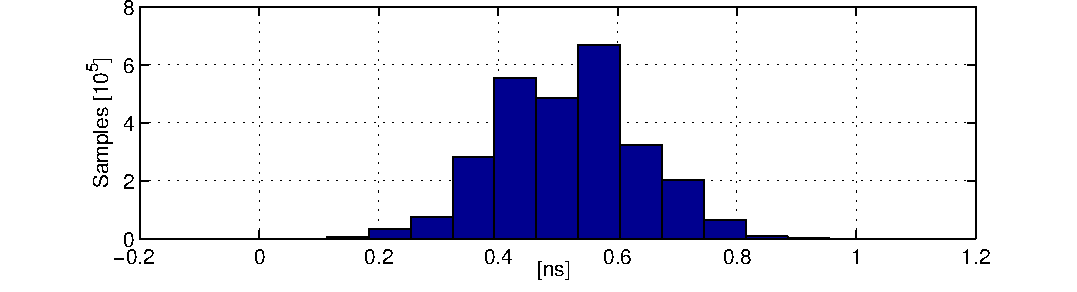
\includegraphics[width=1.1\textwidth]{figs/histogram-small.eps}
		\begin{itemize}
			\item Accuracy: 0.517 ns
			\item Precision: 0.119 ns (std. dev)
		\end{itemize}			


% 	      \begin{table}[!t]\tiny
% 	      \begin{tabular}{| l | c | c |}          \hline
% 	       \multicolumn{3}{|c|}{\textbf{Local PPS }}  \\   \hline
% 	      & \textbf{UTC} & \textbf{nanoseconds} \\   \hline
% 
% 	      1 & 1337380733 & 999999885.959 \\   \hline
% 	      2 & 1337380734 & 999999886.014 \\   \hline
% 	      3 & 1337380735 & 999999885.934 \\   \hline
% 	      4 & 1337380736 & 999999885.906 \\   \hline
% 		&      ...   &  ..           \\   \hline
% 	      2706160 & 1340086893 & 999999885.879 \\   \hline
% 		      
% 	      \end{tabular}
% 	      \label{tab:rawData}
% 	      \end{table}
% 	 \vspace{-0.2cm}
% 	      \begin{table}[!t]\tiny
% 	      \begin{tabular}{| l | c | c |}          \hline 
% 	       \multicolumn{3}{|c|}{\textbf{Loopback PPS}}   \\   \hline
% 	      & \textbf{UTC} & \textbf{nanoseconds} \\   \hline
% 
% 	      1 & 1337380733 & 999999885.500 \\   \hline
% 	      2 & 1337380734 & 999999885.285 \\   \hline
% 	      3 & 1337380735 & 999999885.338 \\   \hline
% 	      4 & 1337380736 & 999999885.420 \\   \hline
% 		&     ..     &      ..       \\   \hline
% 	      2706160 & 1340086893 & 999999885.258 \\   \hline
% 		      
% 	      \end{tabular}
% 	      \label{tab:rawData}
% 	      \end{table}
% 	\vspace{-0.7cm}
% 	      \begin{table}[!t]\tiny
% 	      \begin{tabular}{| l | c| c | c |}          \hline
% 	       \multicolumn{4}{|c|}{\textbf{Time Error}}   \\   \hline
% 	      & \textbf{$x_{lo}$} & \textbf{$x_{lb}$} & \textbf{$x_{diff}$} \\   \hline
% 		    & [ns]  &  [ns]  & [ns]   \\   \hline
% 	      1      & 0.043 & -0.015 & 0.459 \\   \hline
% 	      2      &-0.172 &  0.040 & 0.729 \\   \hline
% 	      3      &-0.119 & -0.040 & 0.596 \\   \hline
% 	      4      &-0.037 & -0.067 & 0.486 \\   \hline
% 	      ...    &  ...  &  ...   &  ...  \\   \hline
% 	      2706160&-0.037 & 0.0671 & 0.621 \\   \hline
% 	      \end{tabular}
% 	      \label{tab:notRawData}
% 	      \end{table}

	  \end{center}
	\column{0.6\textwidth}
		\begin{center}
		\includegraphics[width=0.93\textwidth]{figs/performance_testing_setup-detail.v2.eps}
% 		\hspace{-1cm}
% 		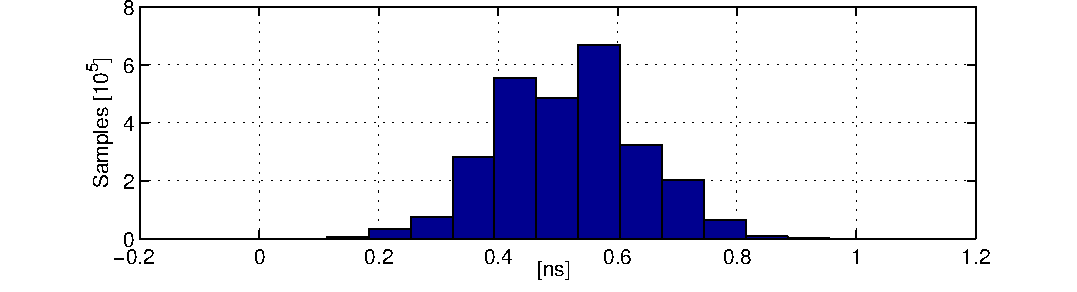
\includegraphics[width=1.1\textwidth]{figs/histogram-small.eps}
% 		\begin{itemize}
% 			\item Accuracy: 0.517 ns
% 			\item Precision: 0.119 ns (std. dev)
% 		\end{itemize}			
		
		
		\end{center}
  \end{columns}


\end{frame}
%%%%%%%%%%%%%%%%%%%%%%%%%%%%%%%%%%%%%%%%%%%%%%%%%%%%%%%%%%%%%%%%%%%%%%%%%%%%%%%%%%%%%%%%%%%%%%%%%%%%
% \section{Temperature Tests}
% \subsection{}
%%%%%%%%%%%%%%%%%%%%%%%%%%%%%%%%%%%%%%%%%%%%%%%%%%%%%%%%%%%%%%%%%%%%%%%%%%%%%%%%%%%%%%%%%%%%%%%%%%%%
\begin{frame}{CNGS performance results (2)}

  \begin{columns}[c]
	\column{0.5\textwidth}
		\begin{center}
		\includegraphics[width=0.9\textwidth]{figs/oADEV3.eps}
		\end{center}
		\begin{center}
		  Overlapping Allan Deviation \\
		  (White or Flicker PM noise)
		\end{center}


	\column{0.6\textwidth}
		\begin{center}
		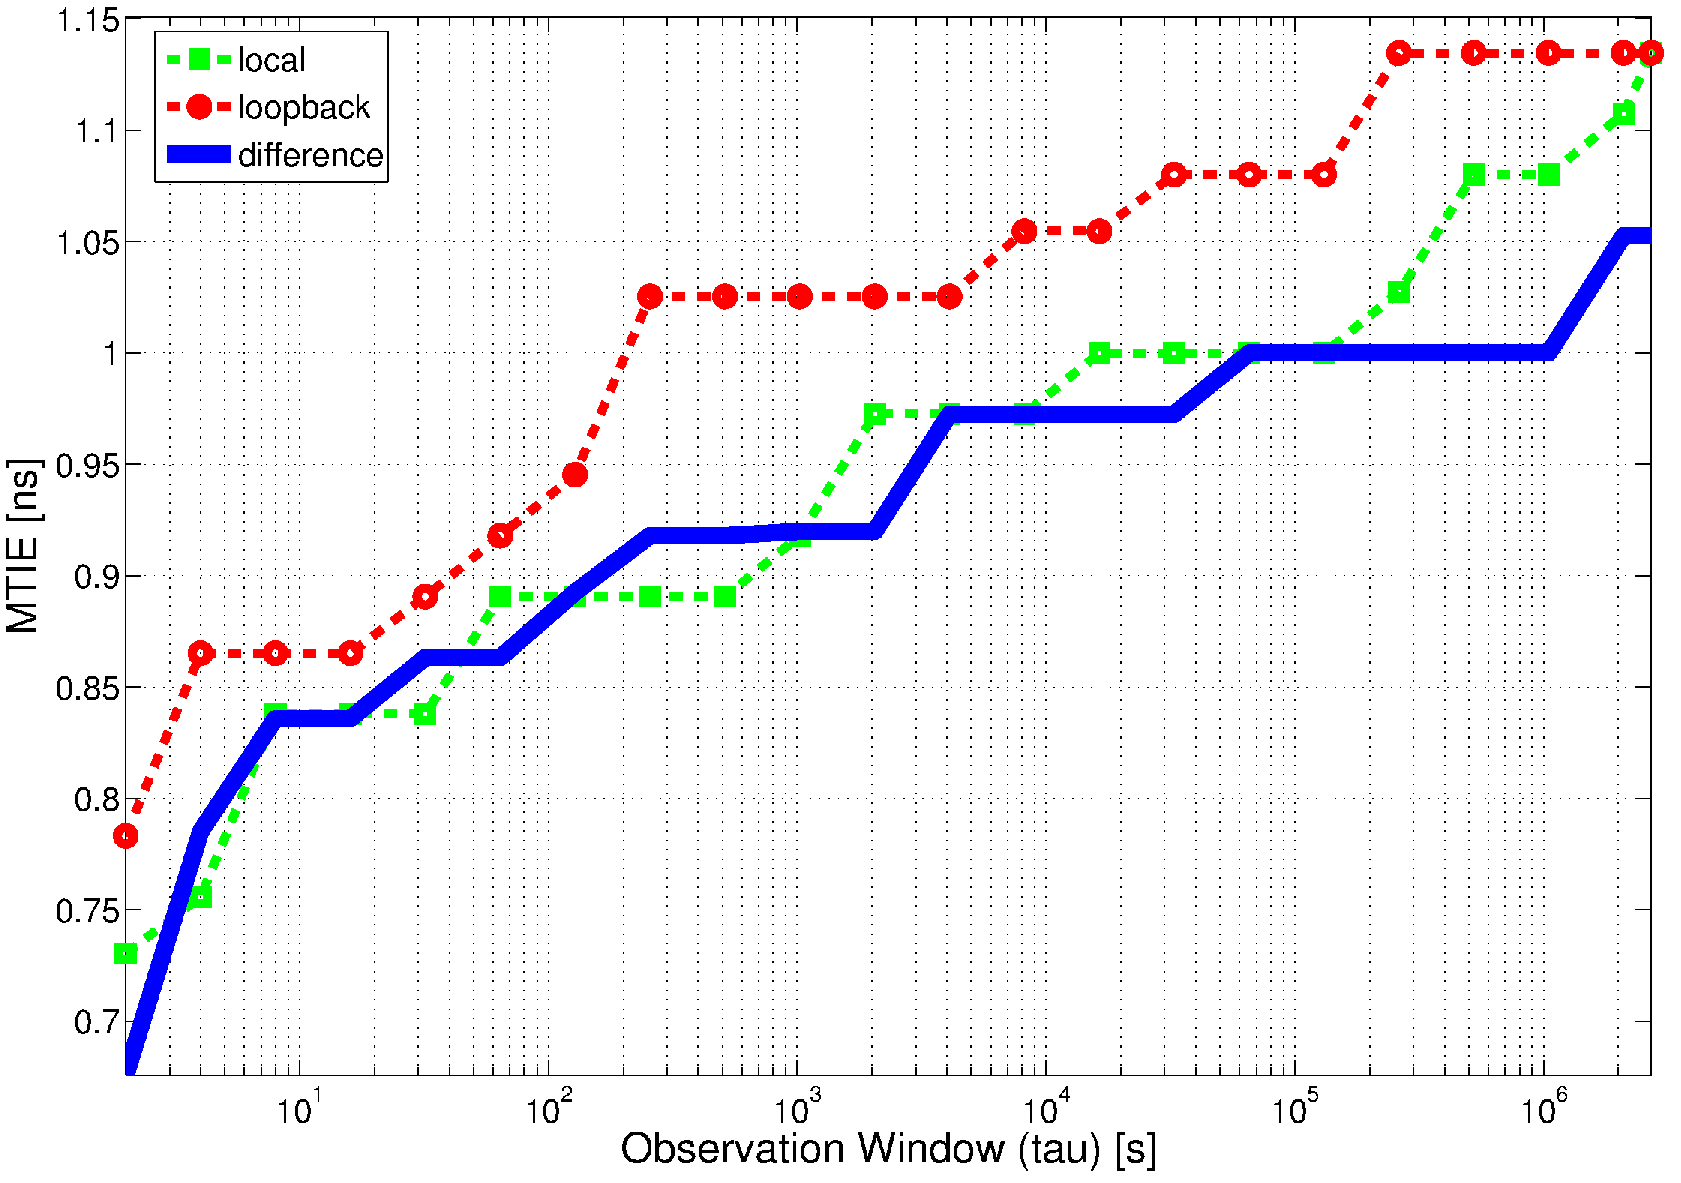
\includegraphics[width=0.9\textwidth]{figs/MTIE2.eps}
		\end{center}
		\begin{center}
		Maximum Time Interval Error
		\end{center}
  \end{columns}
  \begin{columns}[c]
	\column{0.5\textwidth}

	\column{0.6\textwidth}
% 		\begin{center}
% 		      \begin{table}[!t] \tiny
% 		      \begin{tabular}{| c | c | c |}          \hline
% 		      \textcolor{blue}{local}& \textcolor{red}{loopback} & \textcolor{green}{difference}        \\ \hline
% 		      \textcolor{blue}{$\leq$1.15ns}& \textcolor{red}{$\leq$1.15ns} & \textcolor{green}{$\leq$1.05ns}        \\ \hline
% 		      \end{tabular}
% 		      \end{table}   
% 		\end{center}
  \end{columns}

\end{frame}
%%%%%%%%%%%%%%%%%%%%%%%%%%%%%%%%%%%%%%%%%%%%%%%%%%%%%%%%%%%%%%%%%%%%%%%%%%%%%%%%%%%%%%%%%%%%%%%%%%%%
% \section{Temperature Tests}
% \subsection{}
%%%%%%%%%%%%%%%%%%%%%%%%%%%%%%%%%%%%%%%%%%%%%%%%%%%%%%%%%%%%%%%%%%%%%%%%%%%%%%%%%%%%%%%%%%%%%%%%%%%%
\begin{frame}{CNGS performance results (2)}

  \begin{columns}[c]
	\column{0.5\textwidth}
	\begin{center}

	    Out of $2.7*10^6$ samples\\
			\textbf{\textcolor{blue}{~9 values of $x_{diff}$ [0.0003$\%$]}} \\
                       exceeded MTIE=1ns
		
% 
% 	    \textbf{Out of $2.7*10^6$ samples\\ $\pm$ 0.5~ns range exceeded by:}
% 		\begin{itemize}
% 			\item ~~9 values of $x_{diff}$ [0.0003$\%$]
% 			\item ~~25 values of $x_{lo}$ [0.0009$\%$]
% 			\item 146 values of $x_{lb}$  [0.0050$\%$]
% 		\end{itemize}		
	\end{center}
	\column{0.6\textwidth}
		\vspace{0.08cm}
		\begin{center}
		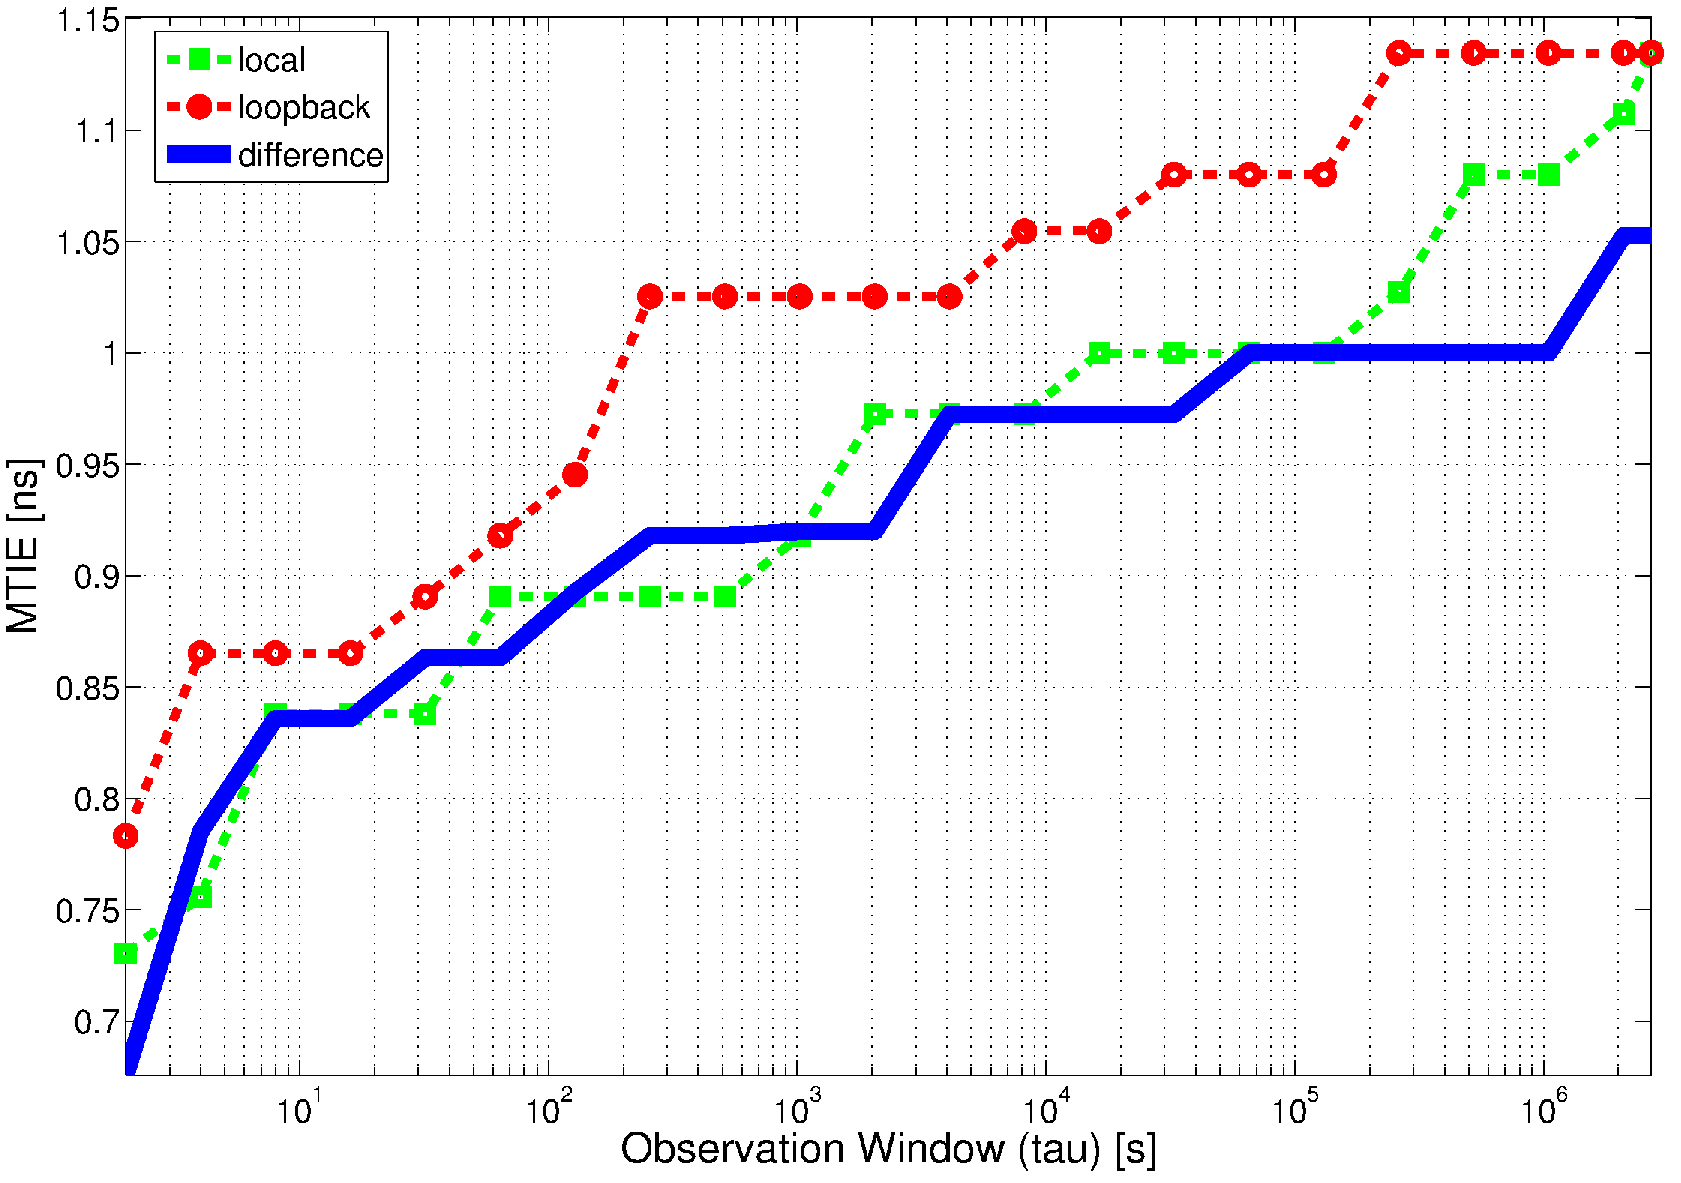
\includegraphics[width=0.9\textwidth]{figs/MTIE2.eps}
		\end{center}
		\begin{center}
		Maximum Time Interval Error
		\end{center}
  \end{columns}
  \begin{columns}[c]
	\column{0.5\textwidth}

	\column{0.6\textwidth}
% 		\begin{center}
% 		      \begin{table}[!t] \tiny
% 		      \begin{tabular}{| c | c | c |}          \hline
% 		      \textcolor{blue}{local}& \textcolor{red}{loopback} & \textcolor{green}{difference}        \\ \hline
% 		      \textcolor{blue}{$\leq$1.15ns}& \textcolor{red}{$\leq$1.15ns} & \textcolor{green}{$\leq$1.05ns}        \\ \hline
% 		      \end{tabular}
% 		      \end{table}   
% 		\end{center}
  \end{columns}
\end{frame}
%%%%%%%%%%%%%%%%%%%%%%%%%%%%%%%%%%%%%%%%%%%%%%%%%%%%%%%%%%%%%%%%%%%%%%%%%%%%%%%%%%%%%%%%%%%%%%%%%%%%
% \section{Temperature Tests}
% \subsection{}
%%%%%%%%%%%%%%%%%%%%%%%%%%%%%%%%%%%%%%%%%%%%%%%%%%%%%%%%%%%%%%%%%%%%%%%%%%%%%%%%%%%%%%%%%%%%%%%%%%%%
\begin{frame}{CNGS performance results (3)}

	\begin{center}
		\includegraphics[height=0.6\textheight]{figs/temp.vs.filteredTE3.eps}
	
		\begin{itemize}
			\item Stable temperature of performance measurement setup
			\item Time Error not correlated with temperature in WR Room
			\item Possibly varying temperature of deployed Nodes
		\end{itemize}	
		
	\end{center}



%   \begin{columns}[c]
% 	\column{0.4\textwidth}
% 		\begin{itemize}
% 			\item Stable temperature of switches/SPECs
% 			\item Time Error not collerated with temperature
% 			\item Test with varying temperature useful
% 		\end{itemize}		
% 	\column{0.7\textwidth}
% 		\begin{center}
% 		\includegraphics[width=1.2\textwidth]{figs/temp.vs.filteredTE3.eps}
% 		\end{center}
%   \end{columns}

\end{frame}

%%%%%%%%%%%%%%%%%%%%%%%%%%%%%%%%%%%%%%%%%%%%%%%%%%%%%%%%%%%%%%%%%%%%%%%%%%%%%%%%%%%%%%%%%%%%%%%%%%%%
\section{Temperature Tests}
\subsection{}
%%%%%%%%%%%%%%%%%%%%%%%%%%%%%%%%%%%%%%%%%%%%%%%%%%%%%%%%%%%%%%%%%%%%%%%%%%%%%%%%%%%%%%%%%%%%%%%%%%%%
\begin{frame}{Temperature tests setup (1)}

	\begin{center}
	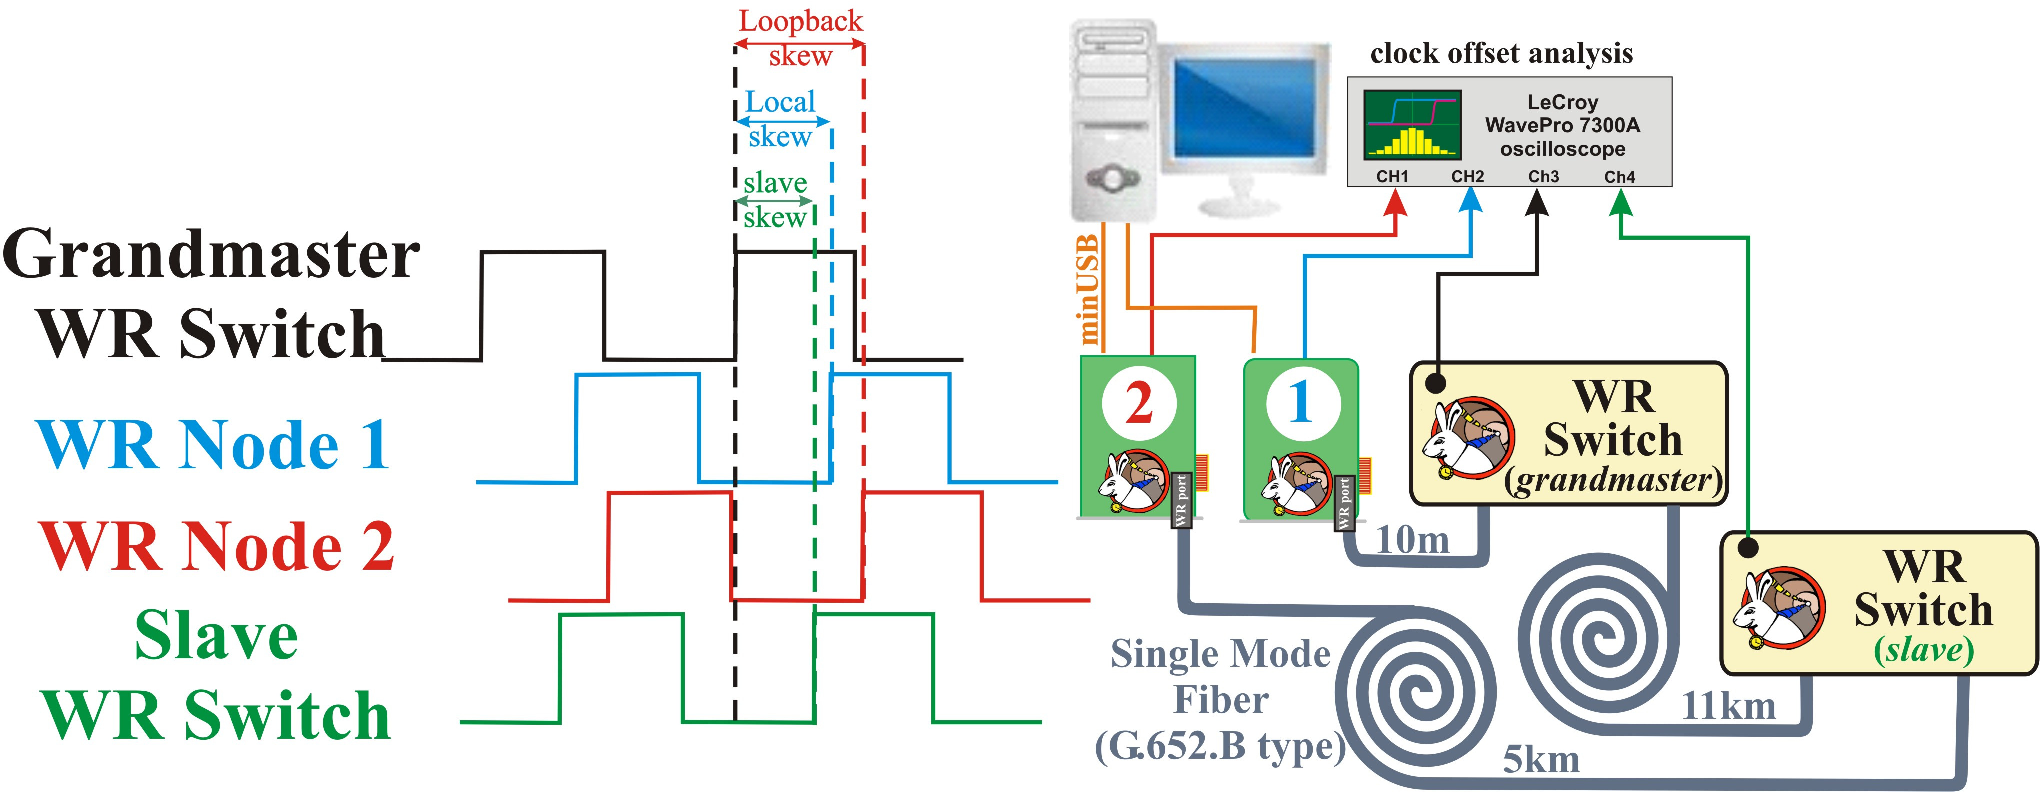
\includegraphics[width=1.0\textwidth]{figs/tempTests-setup.eps}

	\begin{itemize}
		\item Measurement of WR Timebase (clock)
		\item Skew measurement with oscilloscope
	\end{itemize}	

	\end{center}


\end{frame}
%%%%%%%%%%%%%%%%%%%%%%%%%%%%%%%%%%%%%%%%%%%%%%%%%%%%%%%%%%%%%%%%%%%%%%%%%%%%%%%%%%%%%%%%%%%%%%%%%%%%
% \section{Temperature Tests}
% \subsection{}
%%%%%%%%%%%%%%%%%%%%%%%%%%%%%%%%%%%%%%%%%%%%%%%%%%%%%%%%%%%%%%%%%%%%%%%%%%%%%%%%%%%%%%%%%%%%%%%%%%%%
\begin{frame}{Temperature tests setup (2)}

\vspace{-1cm}
  \begin{columns}[c]
	\column{0.5\textwidth}
		\hspace{-1cm}
		\begin{center}
% 		\includegraphics[width=1.0\textwidth]{figs/tempTests-1-temps.eps}
		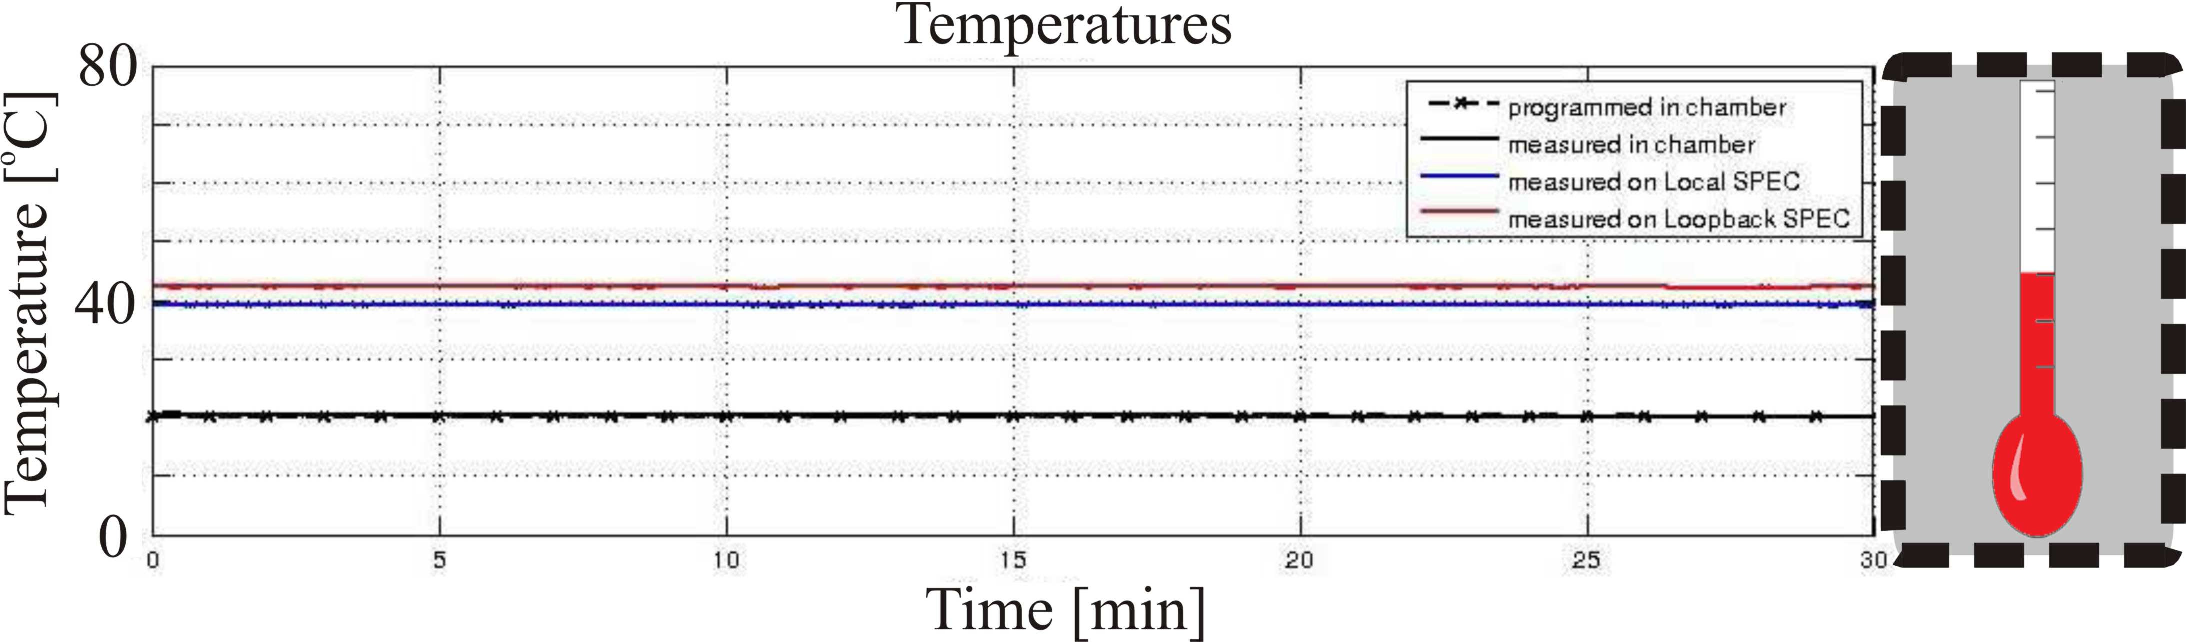
\includegraphics[width=1.0\textwidth]{figs/temp-profile-1.eps}
		\end{center}
\vspace{-0.5cm}
		\begin{center}
		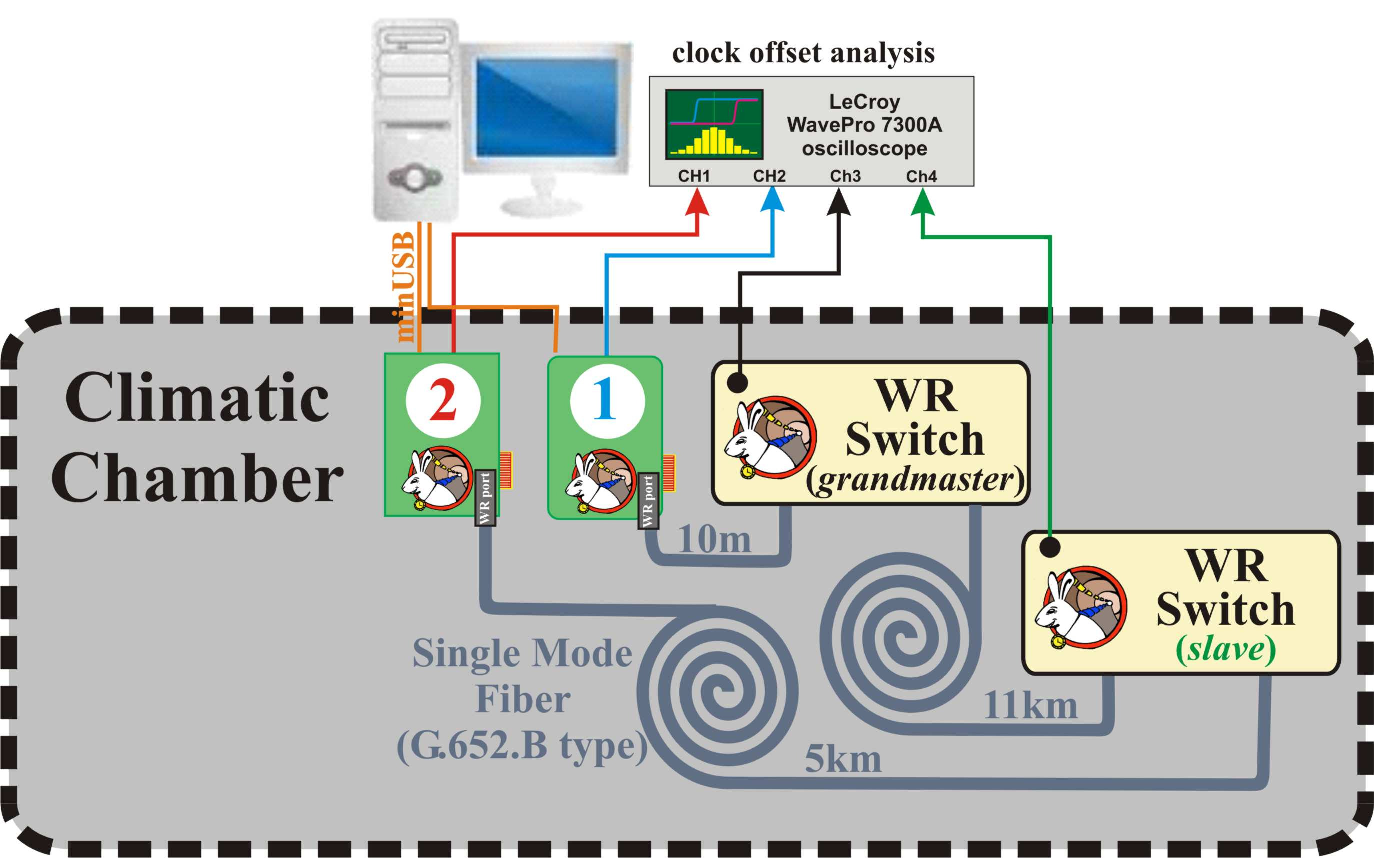
\includegraphics[width=1.0\textwidth]{figs/tempTests-1-setup.eps}
		\end{center}
	\column{0.5\textwidth}
		\hspace{-1cm}
		\begin{center}
% 		\includegraphics[width=1.0\textwidth]{figs/tempTests-2-temps.eps}
		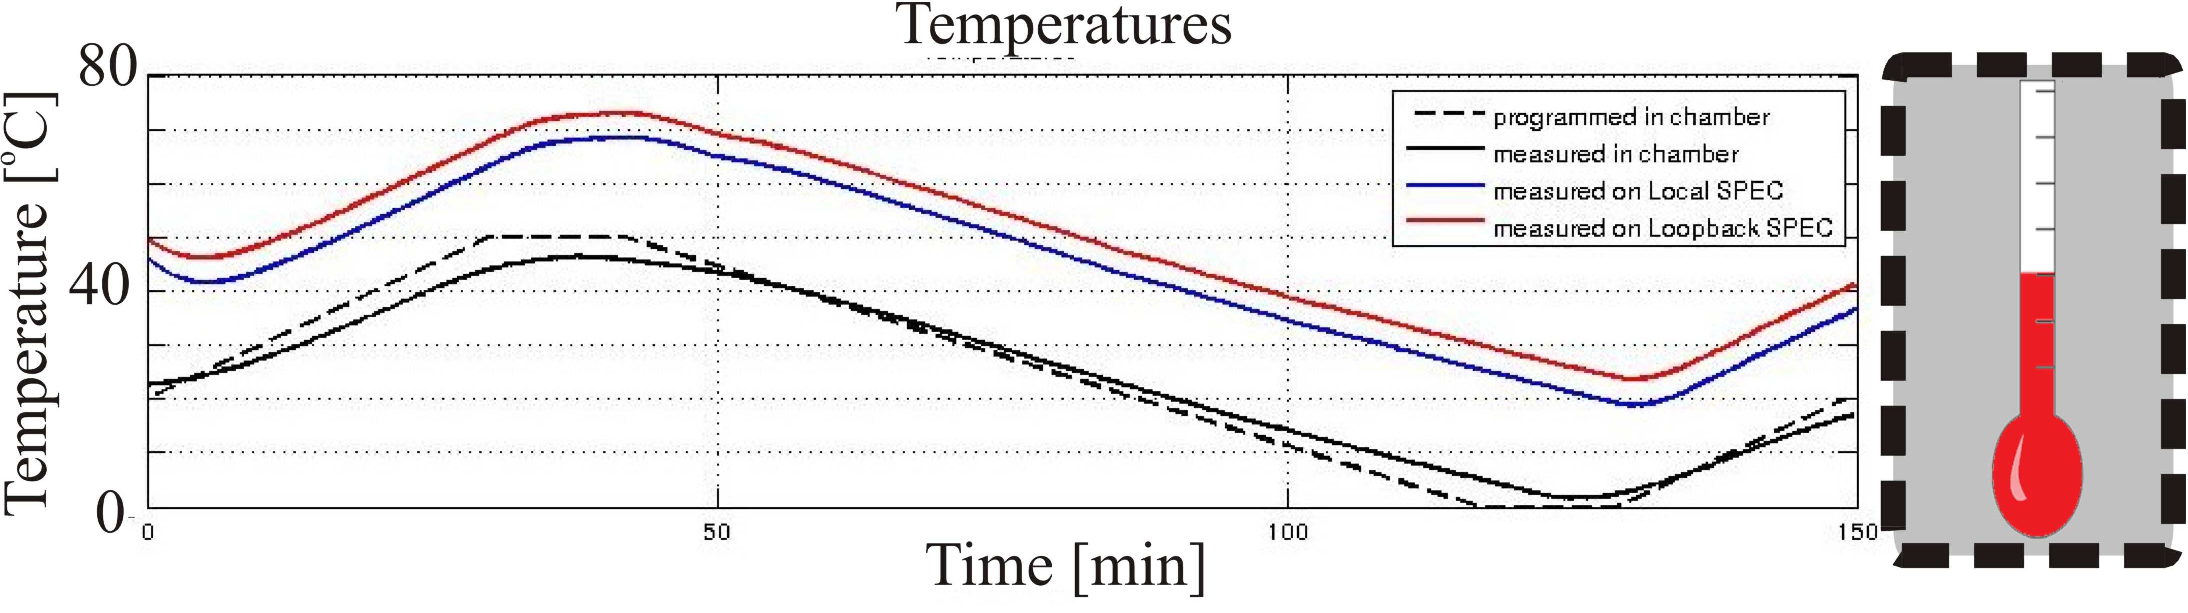
\includegraphics[width=1.0\textwidth]{figs/temp-profile-2.eps}
		\end{center}
		\vspace{-0.5cm}
		\begin{center}
		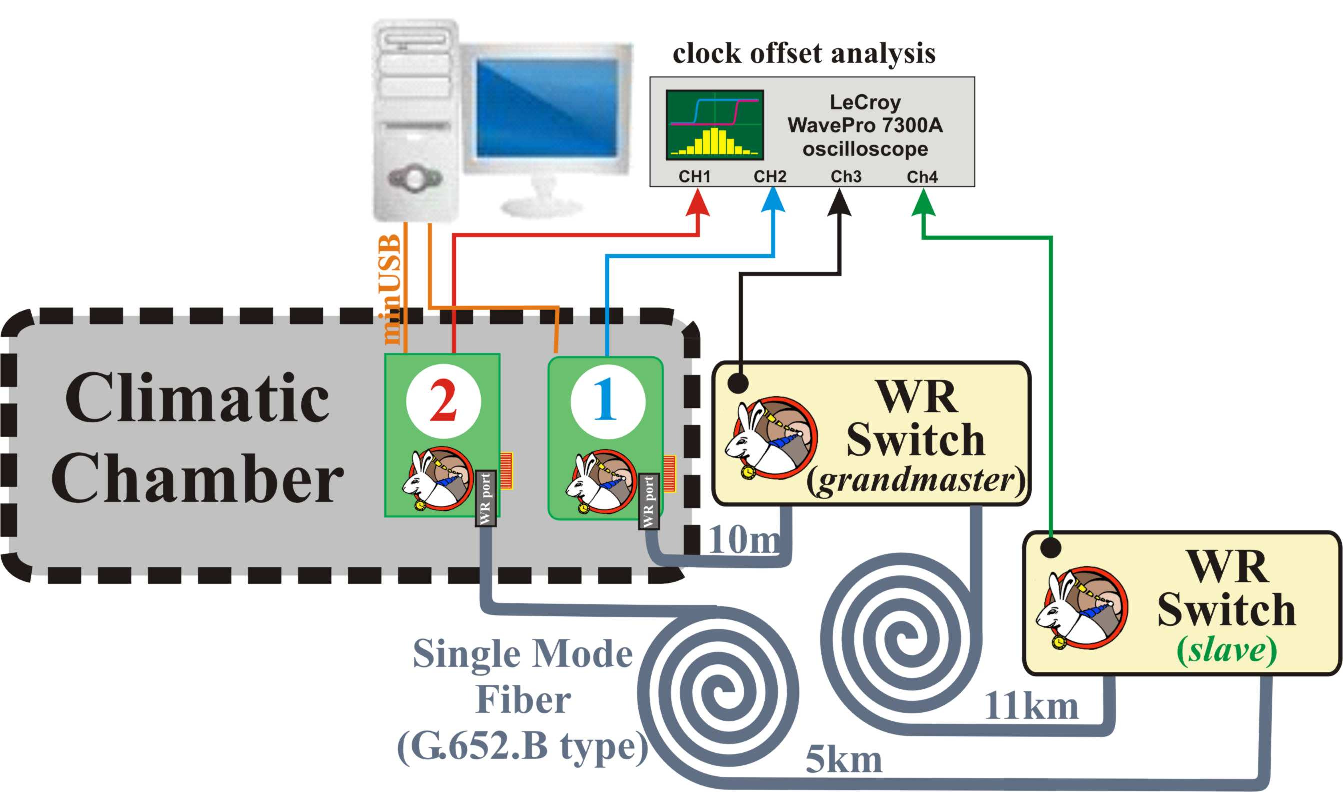
\includegraphics[width=1.0\textwidth]{figs/tempTests-2-setup.eps}
		\end{center}
  \end{columns}

\end{frame}
%%%%%%%%%%%%%%%%%%%%%%%%%%%%%%%%%%%%%%%%%%%%%%%%%%%%%%%%%%%%%%%%%%%%%%%%%%%%%%%%%%%%%%%%%%%%%%%%%%%%
% \section{Temperature Tests}
% \subsection{}
%%%%%%%%%%%%%%%%%%%%%%%%%%%%%%%%%%%%%%%%%%%%%%%%%%%%%%%%%%%%%%%%%%%%%%%%%%%%%%%%%%%%%%%%%%%%%%%%%%%%
% \begin{frame}{Temperature tests results (1)}
% 
% \vspace{-1cm}
%   \begin{columns}[c]
% 	\column{0.5\textwidth}
% 		\hspace{-1cm}
% 		\begin{center}
% 		\includegraphics[width=1.0\textwidth]{figs/tempTests-1-temps.eps}
% 		\end{center}
% 		\vspace{-1cm}
% 		\hspace{-1cm}
% 		\begin{center}
% 		\includegraphics[width=1.0\textwidth]{figs/tempTests-1-hist.eps}
% 		\end{center}
% 		\vspace{-0.8cm}
% 		\begin{center}
% 		      \begin{table}[!t] \tiny
% 		      \begin{tabular}{| l | c |}          \hline 
% 		      \multicolumn{2}{|c|}{\textbf{Stabilized temperature}}       \\ \hline
% 		      \textcolor{blue}{skew sdev [ps]}& \textcolor{blue}{17}       \\ \hline
% 		      \textcolor{red}{skew sdev [ps]} & \textcolor{red}{19}        \\ \hline
% 		      \end{tabular}
% 		      \end{table}   
% 		\end{center}
% 	\column{0.5\textwidth}
% 		\hspace{-1cm}
% 		\begin{center}
% 		\includegraphics[width=1.0\textwidth]{figs/tempTests-2-temps.eps}
% 		\end{center}
% 		\vspace{0.85cm}
% 		\begin{center}
% 		\includegraphics[width=1.0\textwidth]{figs/tempTests-2-hist.eps}
% 		\end{center}
% % 		\vspace{0.2cm}
% 		\begin{center}
% 		      \begin{table}[!t] \tiny
% 		      \begin{tabular}{| l | c |}          \hline
% 		      \multicolumn{2}{|c|}{\textbf{Variable temperature}}           \\ \hline
% 		      \textcolor{blue}{skew sdev [ps]}& \textcolor{blue}{55}        \\ \hline
% 		      \textcolor{red}{skew sdev [ps]} & \textcolor{red}{36}         \\ \hline
% 		      \end{tabular}
% 		      \end{table}   
% 		\end{center}
% 
%   \end{columns}
% 
% 
% 
% \end{frame}
%%%%%%%%%%%%%%%%%%%%%%%%%%%%%%%%%%%%%%%%%%%%%%%%%%%%%%%%%%%%%%%%%%%%%%%%%%%%%%%%%%%%%%%%%%%%%%%%%%%%
% \section{Temperature Tests}
% \subsection{}
%%%%%%%%%%%%%%%%%%%%%%%%%%%%%%%%%%%%%%%%%%%%%%%%%%%%%%%%%%%%%%%%%%%%%%%%%%%%%%%%%%%%%%%%%%%%%%%%%%%%
% \begin{frame}{Temperature tests results (2)}
% 
%   \vspace{-1cm}
%   \begin{columns}[c]
% 	\column{0.5\textwidth}
% 		\hspace{-1cm}
% 		\begin{center}
% 		\includegraphics[width=1.0\textwidth]{figs/tempTests-1-temps.eps}
% 		\end{center}
% 
% 	\column{0.5\textwidth}
% 		\hspace{-1cm}
% 		\begin{center}
% 		\includegraphics[width=1.0\textwidth]{figs/tempTests-2-temps.eps}
% 		\end{center}
%   \end{columns}
% 	\vspace{-0.3cm}
% 	\begin{center}
% 	\includegraphics[width=1.0\textwidth]{figs/tempTests-MTIE.eps}
% 	\end{center}
%   \vspace{-1cm}
%   \begin{columns}[c]
% 	\column{0.5\textwidth}
% 	    \begin{center}
% 		  \begin{table}[!t] \tiny
% 		  \begin{tabular}{| l | c |}          \hline
% 		  \multicolumn{2}{|c|}{\textbf{Stabilized temperature}}       \\ \hline
% 		  \textcolor{blue}{MTIE [ps]}     & \textcolor{blue}{$\leq$203}\\ \hline
% 		  \textcolor{red}{MTIE [ps]}      & \textcolor{red}{$\leq$184} \\ \hline
% 		  \end{tabular}
% 		  \end{table}   
% 	    \end{center}
% 
% 	\column{0.5\textwidth}
% 	     \begin{center}
% 		  \begin{table}[!t] \tiny
% 		  \begin{tabular}{| l | c |}          \hline
% 		  \multicolumn{2}{|c|}{\textbf{Variable temperature}}           \\ \hline
% 		  \textcolor{blue}{MTIE [ps]} & \textcolor{blue}{$\leq$342} \\ \hline
% 		  \textcolor{red}{MTIE [ps]}  & \textcolor{red}{$\leq$289}  \\ \hline
% 		  \end{tabular}
% 		  \end{table}   
% 	    \end{center}
%   \end{columns}
% 
% 
% 
% \end{frame}
%%%%%%%%%%%%%%%%%%%%%%%%%%%%%%%%%%%%%%%%%%%%%%%%%%%%%%%%%%%%%%%%%%%%%%%%%%%%%%%%%%%%%%%%%%%%%%%%%%%%
% \section{Temperature Tests}
% \subsection{}
%%%%%%%%%%%%%%%%%%%%%%%%%%%%%%%%%%%%%%%%%%%%%%%%%%%%%%%%%%%%%%%%%%%%%%%%%%%%%%%%%%%%%%%%%%%%%%%%%%%%
\begin{frame}{Temperature tests results (1)}


  \begin{columns}[c]
	\column{0.5\textwidth}
		\hspace{-1.0cm}
		\begin{center}
		\includegraphics[width=1.1\textwidth]{figs/tempTests-trends.v3.eps}
		\end{center}

		\begin{center}
		  \begin{table}[!t] \footnotesize 
		  \begin{tabular}{ c  c }     
		  \multicolumn{2}{c}{ }       \\         
		   \multicolumn{2}{c}{ }       \\    
		     &    \\ 
		    &     \\ 
		  \end{tabular}
		  \end{table}   		
		\end{center}

	\column{0.5\textwidth}
		\hspace{-0.8cm}
		\begin{center}
		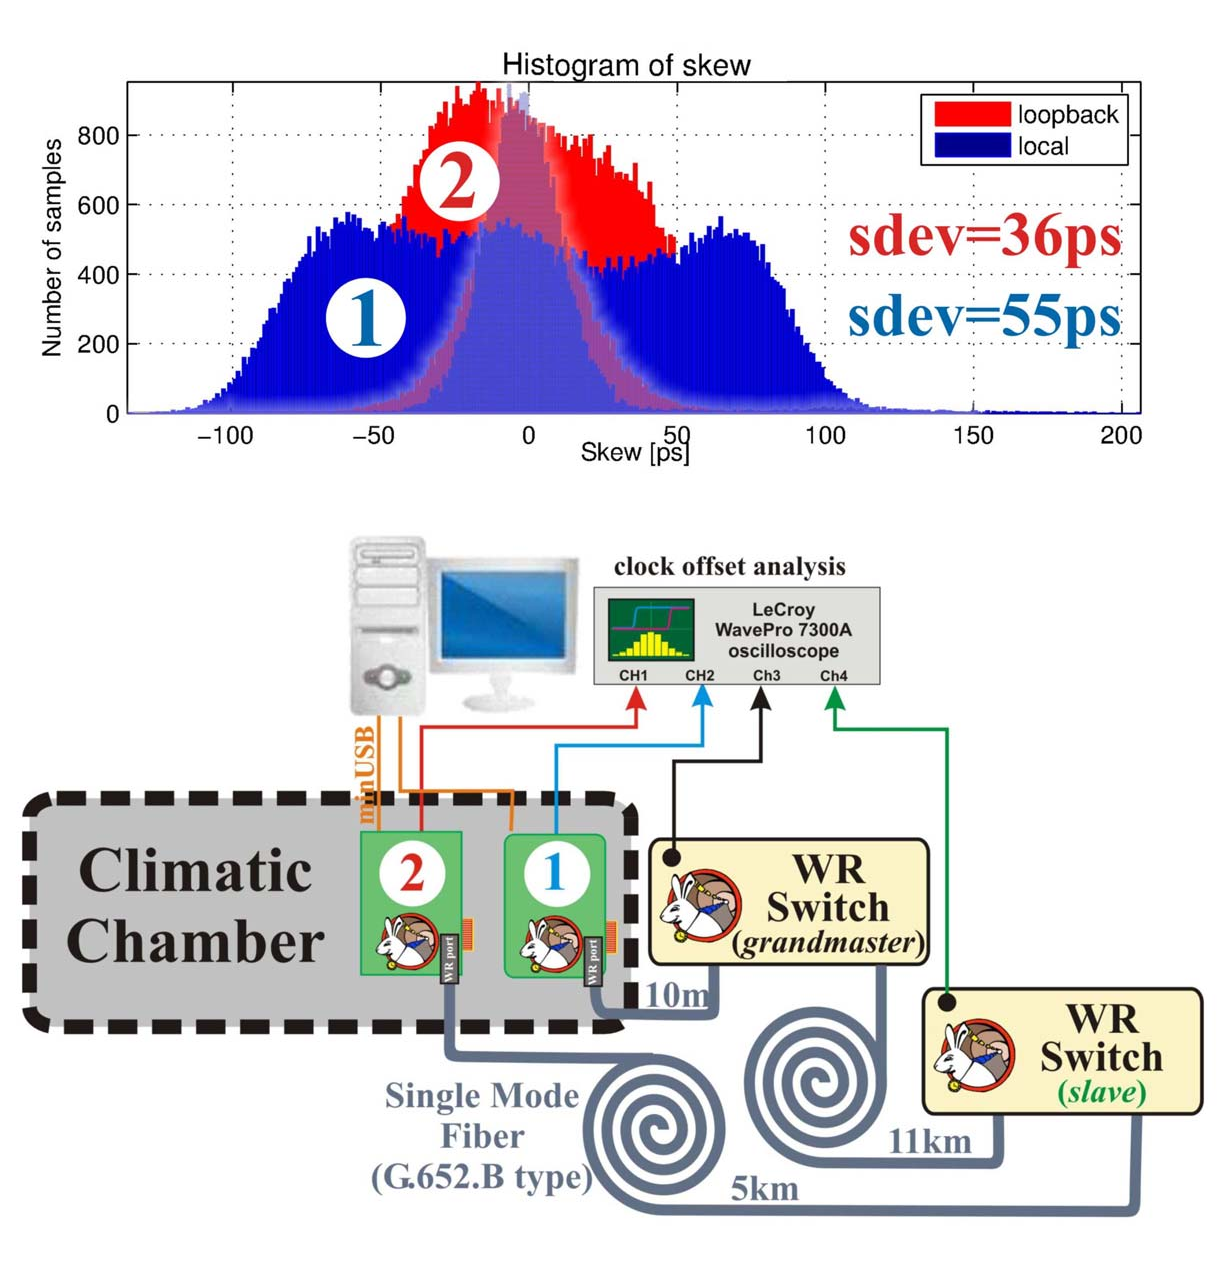
\includegraphics[width=1.13\textwidth]{figs/tempTests-2-combo.eps}
		\end{center}

% 		\vspace{-0.3cm}
% 		\begin{center}
% 		\includegraphics[width=1.0\textwidth]{figs/tempTests-2-hist.v2.eps}
% 		\end{center}
% 		\vspace{-0.8cm}
% 		\begin{center}
% 		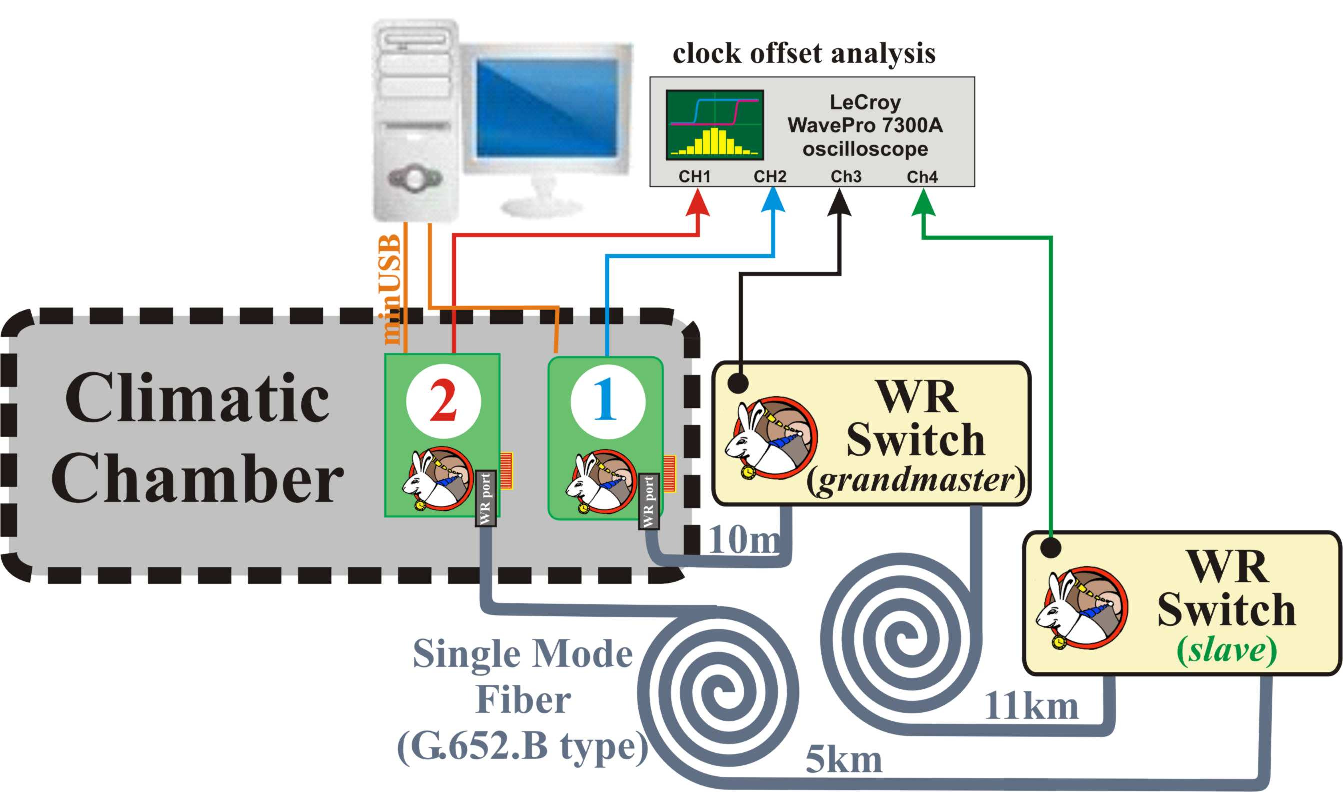
\includegraphics[width=1.0\textwidth]{figs/tempTests-2-setup.eps}
% 		\end{center}
  \end{columns}
%   \vspace{-1cm}
%   \begin{columns}[c]
% 	\column{0.4\textwidth}
% 	    \begin{center}
% 		  \begin{table}[!t] \tiny
% 		  \begin{tabular}{| l | c |}          \hline
% 		  \multicolumn{2}{|c|}{\textbf{Stabilized temperature}}       \\ \hline
% 		  MTIE [ps]                   & skew sdev [ps] \\ \hline
% 		  \textcolor{blue}{$\leq$203} & \textcolor{blue}{17}\\ \hline
% 		  \textcolor{red}{$\leq$184}  & \textcolor{red}{19} \\ \hline
% 		  \end{tabular}
% 		  \end{table}   
% 	    \end{center}
% 	\column{0.2\textwidth}
% 
% 	
% 	\column{0.4\textwidth}
% 	    \begin{center}
% 		  \begin{table}[!t] \tiny
% 		  \begin{tabular}{| l | c |}          \hline
% 		  \multicolumn{2}{|c|}{\textbf{Variable temperature}}       \\ \hline
% 		  MTIE [ps]                   & skew sdev [ps] \\ \hline
% 		  \textcolor{blue}{$\leq$342} & \textcolor{blue}{55}\\ \hline
% 		  \textcolor{red}{$\leq$289}  & \textcolor{red}{36} \\ \hline
% 		  \end{tabular}
% 		  \end{table}   
% 	    \end{center}
%   \end{columns}

\end{frame}
%%%%%%%%%%%%%%%%%%%%%%%%%%%%%%%%%%%%%%%%%%%%%%%%%%%%%%%%%%%%%%%%%%%%%%%%%%%%%%%%%%%%%%%%%%%%%%%%%%%%
% \section{Temperature Tests}
% \subsection{}
%%%%%%%%%%%%%%%%%%%%%%%%%%%%%%%%%%%%%%%%%%%%%%%%%%%%%%%%%%%%%%%%%%%%%%%%%%%%%%%%%%%%%%%%%%%%%%%%%%%%
\begin{frame}{Temperature tests results (2)}


  \begin{columns}[c]
	\column{0.5\textwidth}
		\hspace{-1.0cm}
		\begin{center}
		\includegraphics[width=1.1\textwidth]{figs/tempTests-trends.v3.eps}
		\end{center}

		\begin{center}
% 		  The change of time offset }       \\      
% 		  due to temperature changes}       \\
% 		   \textbf{Node}  \\
% 		  $\approx 4$ ps per $1^{\circ}$C 
		  \begin{table}[!t] \footnotesize 
		  \begin{tabular}{ c  c }    
		  \multicolumn{2}{c}{ The change of time offset }       \\      
		  \multicolumn{2}{c}{ due to temperature changes}       \\    
		  \multicolumn{2}{c}{}       \\  
		  \multicolumn{2}{c}{ $\approx$ \textbf{4 ps per 1}$^{\circ}$\textbf{C}  }       \\  
% 		  \textbf{Switch} & \textbf{Node} \\ 
% 		  $\approx 8$ ps per $1^{\circ}$C  & $\approx 4$ ps per $1^{\circ}$C  \\ 
		  \end{tabular}
		  \end{table}   		
		\end{center}

	\column{0.5\textwidth}
		\hspace{-0.8cm}
		\begin{center}
		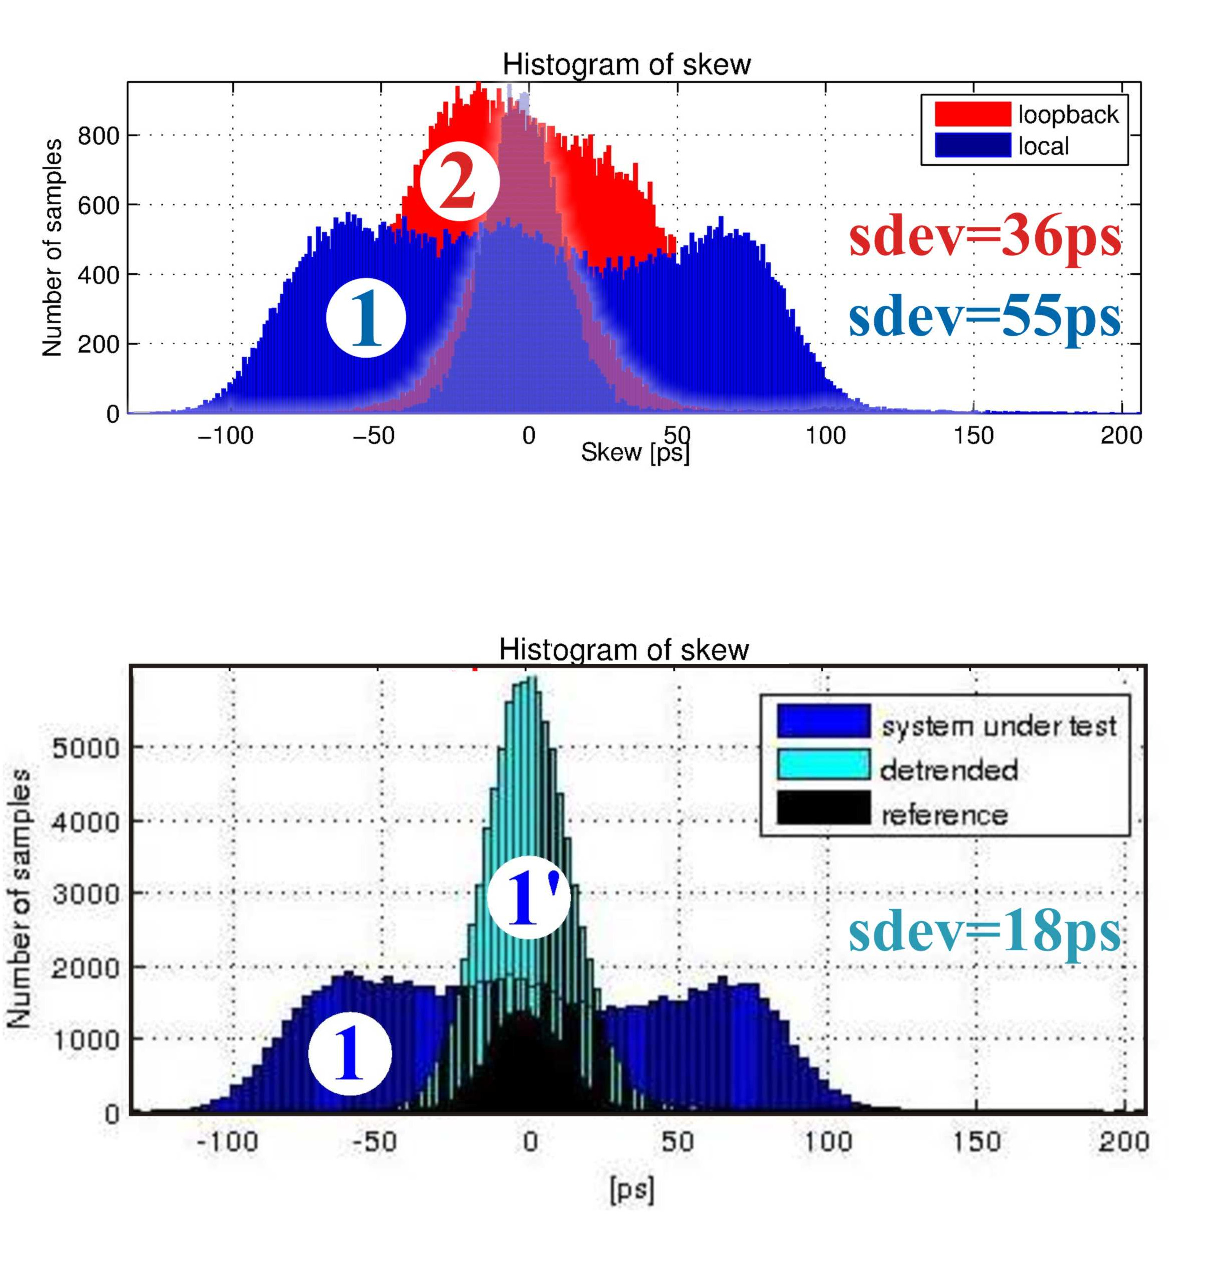
\includegraphics[width=1.13\textwidth]{figs/tempTests-2-combo-detrended.eps}
		\end{center}


% 		\vspace{-0.3cm}
% 		\begin{center}
% 		\includegraphics[width=1.0\textwidth]{figs/tempTests-2-hist-detrended.v2.eps}
% 		\end{center}
% 		\vspace{-1cm}
% 		\begin{center}
% 		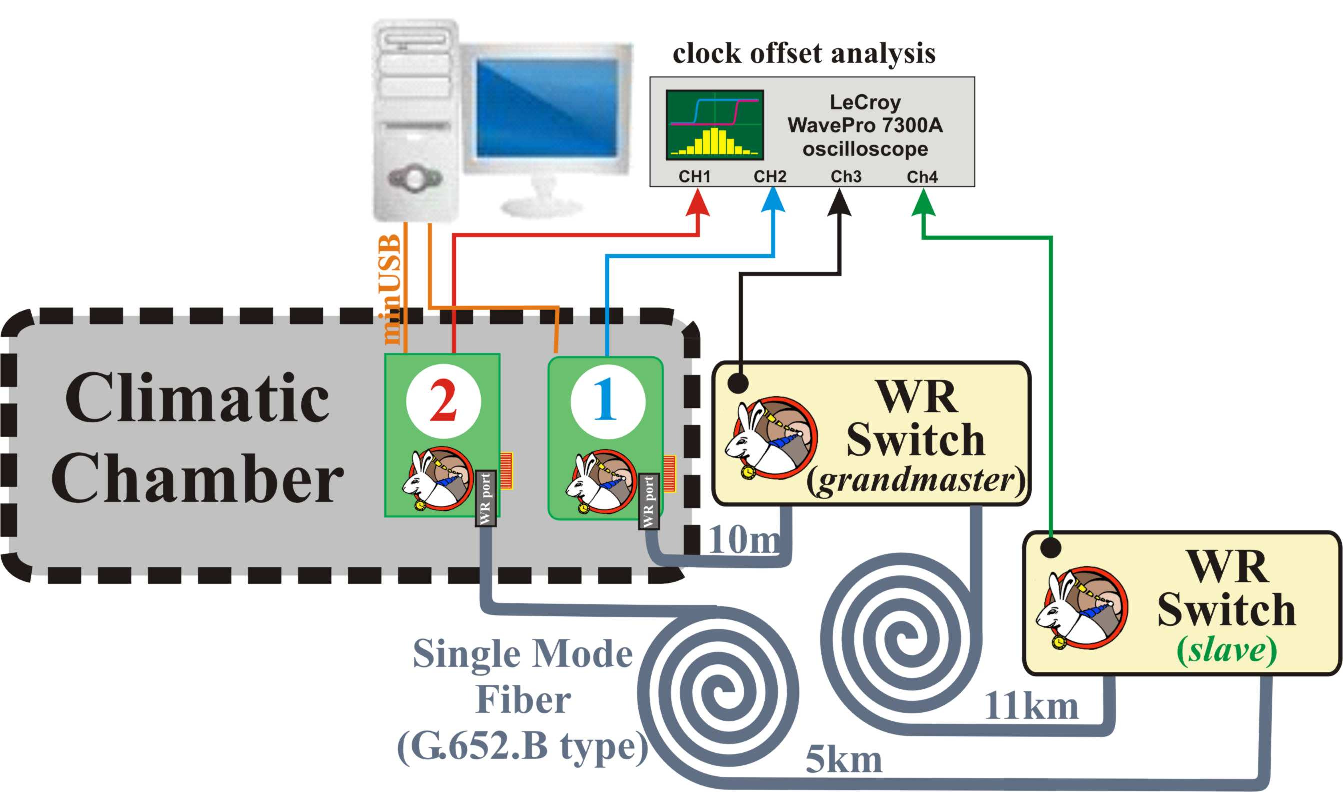
\includegraphics[width=1.0\textwidth]{figs/tempTests-2-setup.eps}
% 		\end{center}
  \end{columns}
%   \vspace{-0.5cm}
%   \begin{columns}[c]
% 	\column{0.4\textwidth}
% 	    \begin{flushright}
% 		  \begin{table}[!t] \tiny
% 		  \begin{tabular}{| l | c |}          \hline
% 		  \multicolumn{2}{|c|}{\textbf{Stabilized temperature}}       \\ \hline
% 		  MTIE [ps]                   & skew sdev [ps] \\ \hline
% 		  \textcolor{blue}{$\leq$203} & \textcolor{blue}{17}\\ \hline
% 		  \textcolor{red}{$\leq$184}  & \textcolor{red}{19} \\ \hline
% 		  \end{tabular}
% 		  \end{table}   
% 	    \end{flushright}
% 	\column{0.2\textwidth}
% 	     \vspace{-0.2cm}
% 	     \hspace{-0.2cm}
% 	     \begin{center}
% 		  \begin{table}[!t] \tiny
% 		  \begin{tabular}{| l | c |}          \hline
% 		  \multicolumn{2}{|c|}{\textbf{Variable temperature}}       \\ 
% 		  \multicolumn{2}{|c|}{\textbf{(linear compensation)}}       \\ \hline
% 		  MTIE [ps]                   & skew sdev [ps] \\ \hline
% 		  \textcolor{blue}{$\leq$247} & \textcolor{blue}{18}\\ \hline
% 		  \end{tabular}
% 		  \end{table}     
% 	    \end{center}
% 	
% 	\column{0.4\textwidth}
% 	    \begin{flushleft}
% 		  \begin{table}[!t] \tiny
% 		  \begin{tabular}{| l | c |}          \hline
% 		  \multicolumn{2}{|c|}{\textbf{Variable temperature}}       \\ \hline
% 		  MTIE [ps]                   & skew sdev [ps] \\ \hline
% 		  \textcolor{blue}{$\leq$342} & \textcolor{blue}{55}\\ \hline
% 		  \textcolor{red}{$\leq$289}  & \textcolor{red}{36} \\ \hline
% 		  \end{tabular}
% 		  \end{table}   
% 	    \end{flushleft}
%   \end{columns}

\end{frame}
%%%%%%%%%%%%%%%%%%%%%%%%%%%%%%%%%%%%%%%%%%%%%%%%%%%%%%%%%%%%%%%%%%%%%%%%%%%%%%%%%%%%%%%%%%%%%%%%%%%%
\section{Conclusions}
\subsection{}
%%%%%%%%%%%%%%%%%%%%%%%%%%%%%%%%%%%%%%%%%%%%%%%%%%%%%%%%%%%%%%%%%%%%%%%%%%%%%%%%%%%%%%%%%%%%%%%%%%%%
\begin{frame}{Conclusions}


%   \begin{columns}[c]
%      \column{0.5\textwidth}
    \begin{itemize}
      \item \textbf{E~=~mc$^2$} 
      \item \textbf{WR-based system} 
      \begin{itemize}
	  \item deployed to verify the speed of neutrinos
	  \item provides nanosecond accuracy
      \end{itemize}
\vspace{0.2cm}
      \item \textbf{WR-timebase} 
      \begin{itemize}
	  \item sub-ns accuracy 
	  \item tens of picoseconds precision 
          \item wide range of temperatures
      \end{itemize}
\vspace{0.2cm}
      \item \textbf{Possible compensation of WR Node's temperature variation}
\vspace{0.1cm}
      \item \textbf{Important milestone in the White Rabbit Project}

    \end{itemize}

%   \column{0.5\textwidth}
%   \end{columns}


\end{frame}
%%%%%%%%%%%%%%%%%%%%%%%%%%%%%%%%%%%%%%%%%%%%%%%%%%%%%%%%%%%%%%%%%%%%%%%%%%%%%%%%%%%%%%%%%%%%%%%%%%%%
% \section{Conclusions}
% \subsection{}
%%%%%%%%%%%%%%%%%%%%%%%%%%%%%%%%%%%%%%%%%%%%%%%%%%%%%%%%%%%%%%%%%%%%%%%%%%%%%%%%%%%%%%%%%%%%%%%%%%%%
% \begin{frame}{Conclusions}
% 
% 
% \end{frame}

%%%%%%%%%%%%%%%%%%%%%%%%%%%%%%%%%%%%%%%%%%%%%%%%%%%%%%%%%%%%%%%%%%%%%%%%%%%%%%%%%%%%%%%%%%%%%%%%%%%%
\section{Q\&A}
\subsection{}
%%%%%%%%%%%%%%%%%%%%%%%%%%%%%%%%%%%%%%%%%%%%%%%%%%%%%%%%%%%%%%%%%%%%%%%%%%%%%%%%%%%%%%%%%%%%%%%%%%%%
\begin{frame}{Questions and answers}

    \begin{center}
    \includegraphics[height=3.5cm]{../../figures/logo/WRlogo.ps}
    \end{center}
    \begin{center}
    \textit{"I don't answer faster-than-light-neutrinos questions"} - said the presented \\
    A neutrino walks into the room...
    \end{center}

\end{frame}


\appendix
\backupbegin

%%%%%%%%%%%%%%%%%%%%%%%%%%%%%%%%%%%%%%%%%%%%%%%%%%%%%%%%%%%%%%%%%%%%%%%%%%%%%%%%%%%%%%%%%%%%%%%%%%%%
%\section{extras}
% \subsection{}
%%%%%%%%%%%%%%%%%%%%%%%%%%%%%%%%%%%%%%%%%%%%%%%%%%%%%%%%%%%%%%%%%%%%%%%%%%%%%%%%%%%%%%%%%%%%%%%%%%%%
\begin{frame}{Extras}

    \begin{center}
      Extras
    \end{center}

\end{frame}
%%%%%%%%%%%%%%%%%%%%%%%%%%%%%%%%%%%%%%%%%%%%%%%%%%%%%%%%%%%%%%%%%%%%%%%%%%%%%%%%%%%%%%%%%%%%%%%%%%%%
\section{Timestamps}
\subsection{}
%%%%%%%%%%%%%%%%%%%%%%%%%%%%%%%%%%%%%%%%%%%%%%%%%%%%%%%%%%%%%%%%%%%%%%%%%%%%%%%%%%%%%%%%%%%%%%%%%%%%
\begin{frame}{Fine Delay Measurement}

  \begin{center}
  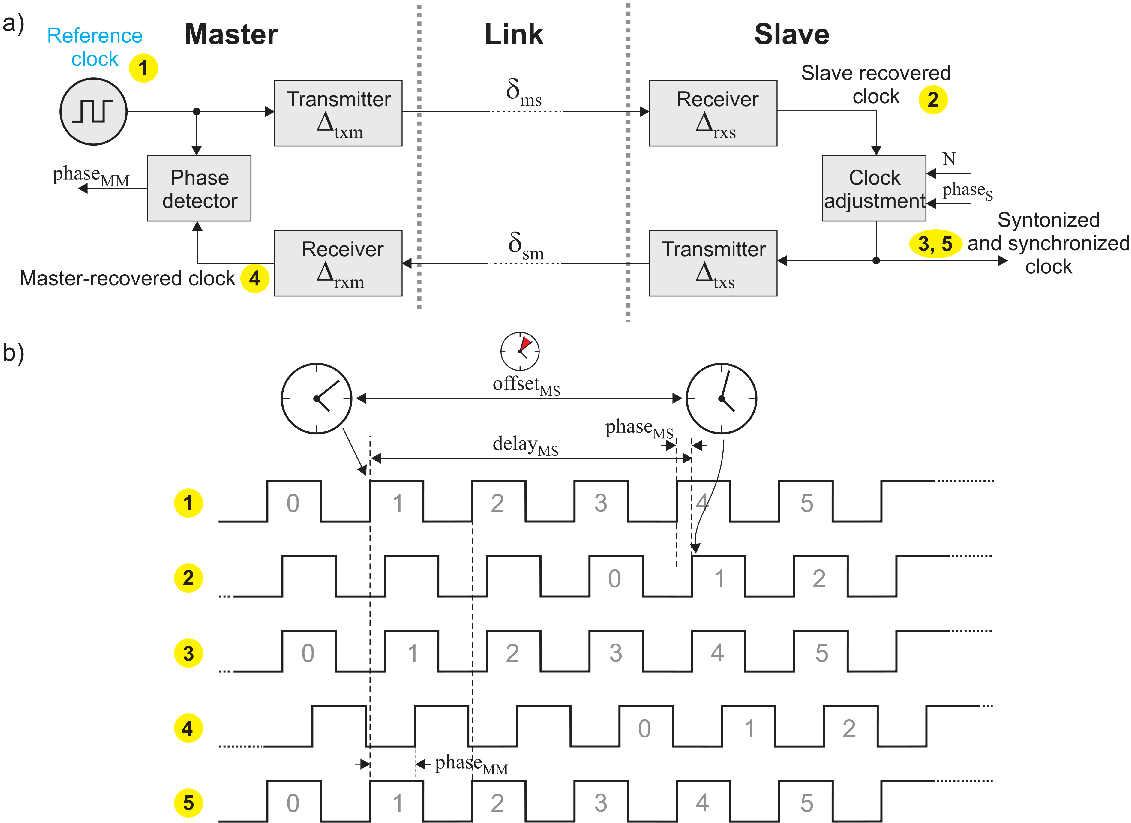
\includegraphics[width=10.0cm]{figs/link_model.eps}
  \end{center}

\end{frame}
%%%%%%%%%%%%%%%%%%%%%%%%%%%%%%%%%%%%%%%%%%%%%%%%%%%%%%%%%%%%%%%%%%%%%%%%%%%%%%%%%%%%%%%%%%%%%%%%%%%%
\section{WR applications}
\subsection{}
%%%%%%%%%%%%%%%%%%%%%%%%%%%%%%%%%%%%%%%%%%%%%%%%%%%%%%%%%%%%%%%%%%%%%%%%%%%%%%%%%%%%%%%%%%%%%%%%%%%%
\begin{frame}{White Rabbit applications}
\begin{center}
   \includegraphics<1>[width=0.80\textwidth]{../../figures/applications/OperaTiming2.eps}
     \end{center}  

\end{frame}

%%%%%%%%%%%%%%%%%%%%%%%%%%%%%%%%%%%%%%%%%%%%%%%%%%%%%%%%%%%%%%%%%%%%%%%%%%%%%%%%%%%%%%%%%%%%%%%%%%%%
\section{WR applications}
\subsection{}
%%%%%%%%%%%%%%%%%%%%%%%%%%%%%%%%%%%%%%%%%%%%%%%%%%%%%%%%%%%%%%%%%%%%%%%%%%%%%%%%%%%%%%%%%%%%%%%%%%%%
\begin{frame}{White Rabbit applications}

\begin{columns}[c]
  \column{0.65\textwidth}

    \begin{itemize}
      \item<1-> Existing applications:
      \begin{itemize}
	\item<1-> \textbf<1>{CERN Neutrinos to Gran Sasso}
      \end{itemize} 
      \item<2-> Future applications:
      \begin{itemize}
	\item<2-> \textbf<2>{CERN and GSI  }
	\item<3-> \textbf<3>{HiSCORE: Gamma\&Cosmic-Ray experiment (Tunka, Siberia)}
	\item<4-> \textbf<4>{The Large High Altitude Air Shower Observatory (Tibet)}
      \end{itemize}         	
      \item<5-> Potential applications:
      \begin{itemize}
	\item<5-> \textbf<5>{Cherenkov Telescope Array}
	\item<6-> \textbf<6>{ITER}
	\item<7> \textbf<7>{European deep-sea research infrastructure (KM3NET)}
      \end{itemize}         	
    \end{itemize}    

  \column{0.55\textwidth}         


    \begin{center}
      \includegraphics<1>[width=0.80\textwidth]{../../figures/applications/OperaTiming2.eps} \pause
      \includegraphics<2>[width=0.6\textwidth]{../../figures/applications/gsiANDcern.eps}   \pause
      \includegraphics<3>[width=0.85\textwidth]{../../figures/applications/tunka.eps}        \pause
      \includegraphics<4>[width=0.85\textwidth]{../../figures/applications/lhaaso.eps}       \pause
      \includegraphics<5>[width=0.85\textwidth]{../../figures/applications/cta.eps}          \pause
      \includegraphics<6>[width=0.85\textwidth]{../../figures/applications/iter.eps}         \pause
      \includegraphics<7>[width=0.85\textwidth]{../../figures/applications/KM3NeT.eps}       
    \end{center}

  \column{0.6\textwidth}         
\end{columns}
\end{frame}

%%%%%%%%%%%%%%%%%%%%%%%%%%%%%%%%%%%%%%%%%%%%%%%%%%%%%%%%%%%%%%%%%%%%%%%%%%%%%%%%%%%%%%%%%%%%%%%%%%%%
\section{Motivation}
\subsection{}
%%%%%%%%%%%%%%%%%%%%%%%%%%%%%%%%%%%%%%%%%%%%%%%%%%%%%%%%%%%%%%%%%%%%%%%%%%%%%%%%%%%%%%%%%%%%%%%%%%%%
\begin{frame}{Why White Rabbit ?}

\begin{columns}[c]
  \column{0.55\textwidth}

    \begin{itemize}
	\item Renovation of General Machine Timing (GMT)
\small
	\item GMT is great but...:
	      \begin{itemize}
		  \item \textbf{RS-422}, 500kbps
		  \item \textbf{Unidirectional} communication
		  \item Separate network required
		  \item \textbf{Custom design, complicated maintenance}
	      \end{itemize}
	\item White Rabbit is meant to solve these problems
    \end{itemize}

  \column{0.6\textwidth}

      \begin{center}
      \includegraphics<1>[width=1.0\textwidth]{../../figures/misc/GMT-1.eps} \pause
      \includegraphics<2>[width=1.0\textwidth]{../../figures/misc/GMT-2.eps} \pause
      \includegraphics<3>[width=1.0\textwidth]{../../figures/misc/GMT2WR.eps}
      \end{center}

\end{columns}

\end{frame}

%%%%%%%%%%%%%%%%%%%%%%%%%%%%%%%%%%%%%%%%%%%%%%%%%%%%%%%%%%%%%%%%%%%%%%%%%%%%%%%%%%%%%%%%%%%%%%%%%%%%
\section{WR Network}
\subsection{}
%%%%%%%%%%%%%%%%%%%%%%%%%%%%%%%%%%%%%%%%%%%%%%%%%%%%%%%%%%%%%%%%%%%%%%%%%%%%%%%%%%%%%%%%%%%%%%%%%%%%
\begin{frame}{Time distribution in White Rabbit}



    \begin{center}
    \includegraphics[height=0.8\textheight]{../../figures/network/wr_network-new.ps}
    \end{center}

\end{frame}

%%%%%%%%%%%%%%%%%%%%%%%%%%%%%%%%%%%%%%%%%%%%%%%%%%%%%%%%%%%%%%%%%%%%%%%%%%%%%%%%%%%%%%%%%%%%%%%%%%%%
\section{System Components}
\subsection{}
%%%%%%%%%%%%%%%%%%%%%%%%%%%%%%%%%%%%%%%%%%%%%%%%%%%%%%%%%%%%%%%%%%%%%%%%%%%%%%%%%%%%%%%%%%%%%%%%%%%%
\begin{frame}{White Rabbit Network Components}


    \begin{center}
    %\includegraphics<1>[width=1.0\textwidth]{fig/WRNcomponents.eps}  \pause
    \includegraphics<1>[width=1.0\textwidth]{../../figures/network/WRnetwork-eva.eps}  \pause
    \includegraphics<2>[width=1.0\textwidth]{../../figures/network/WRNcomponents-1.eps} \pause
    \includegraphics<3>[width=1.0\textwidth]{../../figures/network/WRNcomponents-2.eps}
    \end{center}

\end{frame}
%%%%%%%%%%%%%%%%%%%%%%%%%%%%%%%%%%%%%%%%%%%%%%%%%%%%%%%%%%%%%%%%%%%%%%%%%%%%%%%%%%%%%%%%%%%%%%%%%%%%
%\section{}
%\subsection{Topology Redundancy}
%%%%%%%%%%%%%%%%%%%%%%%%%%%%%%%%%%%%%%%%%%%%%%%%%%%%%%%%%%%%%%%%%%%%%%%%%%%%%%%%%%%%%%%%%%%%%%%%%%%%
\begin{frame}{White Rabbit Switch (V3)}

    \begin{center}
    \includegraphics[width=6.0cm]{../../figures/switch/wrSwitchV3.ps}
    \end{center}

	\begin{itemize}
	\item Central element of WR network
	\item Original design optimized for timing, designed from scratch
	\item 18 1000BASE-BX10 ports
	\item Capable of driving 10 km of SM fiber
	\item Open design (H/W and S/W)
%	\item 200 ps synchronization accuracy
	\end{itemize}

\end{frame}
%%%%%%%%%%%%%%%%%%%%%%%%%%%%%%%%%%%%%%%%%%%%%%%%%%%%%%%%%%%%%%%%%%%%%%%%%%%%%%%%%%%%%%%%%%%%%%%%%%%%
%\section{}
%\subsection{Topology Redundancy}
%%%%%%%%%%%%%%%%%%%%%%%%%%%%%%%%%%%%%%%%%%%%%%%%%%%%%%%%%%%%%%%%%%%%%%%%%%%%%%%%%%%%%%%%%%%%%%%%%%%%
\begin{frame}{WR Node: WR PTP Core}

    \begin{center}
    \includegraphics<1>[width=1.0\textwidth]{../../figures/node/wrpc_box.eps} \pause
    \includegraphics<2>[width=1.0\textwidth]{../../figures/node/wrpc_inside.eps}
    \end{center}

\end{frame}
%%%%%%%%%%%%%%%%%%%%%%%%%%%%%%%%%%%%%%%%%%%%%%%%%%%%%%%%%%%%%%%%%%%%%%%%%%%%%%%%%%%%%%%%%%%%%%%%%%%%
%\section{}
%\subsection{Topology Redundancy}
%%%%%%%%%%%%%%%%%%%%%%%%%%%%%%%%%%%%%%%%%%%%%%%%%%%%%%%%%%%%%%%%%%%%%%%%%%%%%%%%%%%%%%%%%%%%%%%%%%%%
\begin{frame}{WR Node: SPEC board}

    \begin{center}
    \includegraphics[width=7cm]{../../figures/node/shw_kit-1}
    \end{center}

  \begin{columns}[c]
    \column{.01\textwidth}
    \column{.98\textwidth}

	\begin{block}{Co-HT FMC-based Hardware Kit:}
%	\textbf{Co-HT FMC-based Hardware Kit:}
	  \begin{itemize}
	  \item FMCs (FPGA Mezzanine Cards) with ADCs, DACs, TDCs, fine delays, digital I/O
	  \item Carrier boards in PCI-Express, VME and uTCA formats
	  \item All carriers are equipped with a White Rabbit port
	  \end{itemize}
	\end{block}

    \column{.01\textwidth}
  \end{columns}


\end{frame}

%%%%%%%%%%%%%%%%%%%%%%%%%%%%%%%%%%%%%%%%%%%%%%%%%%%%%%%%%%%%%%%%%%%%%%%%%%%%%%%%%%%%%%%%%%%%%%%%%%%%
%\section{}
%\subsection{Topology Redundancy}
%%%%%%%%%%%%%%%%%%%%%%%%%%%%%%%%%%%%%%%%%%%%%%%%%%%%%%%%%%%%%%%%%%%%%%%%%%%%%%%%%%%%%%%%%%%%%%%%%%%%
\begin{frame}{WR Node: SPEC board}

    \begin{center}
    \includegraphics[width=1.0\textwidth]{../../figures/node/specInterior.eps}
    \end{center}

\end{frame}

%%%%%%%%%%%%%%%%%%%%%%%%%%%%%%%%%%%%%%%%%%%%%%%%%%%%%%%%%%%%%%%%%%%%%%%%%%%%%%%%%%%%%%%%%%%%%%%%%%%%
%\section{}
%\subsection{Topology Redundancy}
%%%%%%%%%%%%%%%%%%%%%%%%%%%%%%%%%%%%%%%%%%%%%%%%%%%%%%%%%%%%%%%%%%%%%%%%%%%%%%%%%%%%%%%%%%%%%%%%%%%%
\begin{frame}{WR Node: ongoing efforts}


  \begin{columns}[c]
    \column{.7\textwidth}
\small
      \begin{itemize}
        \item \textbf<1>{Simple VME FMC Carrier (SVEC)}
        \item \textbf<2>{Compact Universal Timing Endpoint Based on White Rabbit}
        \item \textbf<3>{WR-compatible multi-FMC carrier}
	\item \textbf<4>{PXI express FMC Carrier Board (SPEXI)}
      \end{itemize}

    
    \begin{center}
       \textcolor{gray}{www.ohwr.org/projects/spexi/wiki}
    \end{center}


    \column{.5\textwidth}

    \begin{center}
      \includegraphics<1>[width=0.9\textwidth]{../../figures/node/svec4_res.eps} \pause
      \includegraphics<2>[width=0.7\textwidth]{../../figures/node/stm.eps}       \pause
      \includegraphics<3>[width=0.9\textwidth]{../../figures/node/WRCarrier.eps} \pause
      \includegraphics<4>[width=0.5\textwidth]{../../figures/node/pxi.eps} 
    \end{center}

    \column{.01\textwidth}
  \end{columns}

%     \begin{center}
%     \includegraphics<1>[width=1.0\textwidth]{fig/stm.eps}       \pause
%     \includegraphics<2>[width=1.0\textwidth]{fig/svec4_res.eps} \pause
%     \includegraphics<3>[width=1.0\textwidth]{fig/WRCarrier.eps}
%     \end{center}

\end{frame}

\backupend

%%%%%%%%%%%%%%%%%%%%%%%%%%%%%%%%%%%%%%%%%%%%%%%%%%%%%%%%%%%%%%%%%%%%%%%%%%%%%%%%%%%%%%%%%%%%%%%%%%%%%%%
\end{document}
%%%%%%%%%%%%%%%%%%%%%%%%%%%%%%%%%%%%%%%%%%%%%%%%%%%%%%%%%%%%%%%%%%%%%%%%%%%%%%%%%%%%%%%%%%%%%%%%%%%%%%%